%!TEX TS-program = xelatex
%!TEX encoding = UTF-8 Unicode
% Awesome CV LaTeX Template for CV/Resume
%
% This template has been downloaded from:
% https://github.com/posquit0/Awesome-CV
%
% Author:
% Claud D. Park <posquit0.bj@gmail.com>
% http://www.posquit0.com
%
%
% Adapted to be an Rmarkdown template by Mitchell O'Hara-Wild
% 23 November 2018
%
% Template license:
% CC BY-SA 4.0 (https://creativecommons.org/licenses/by-sa/4.0/)
%
%-------------------------------------------------------------------------------
% CONFIGURATIONS
%-------------------------------------------------------------------------------
% A4 paper size by default, use 'letterpaper' for US letter
\documentclass[11pt,a4paper,]{awesome-cv}

% Configure page margins with geometry
\usepackage{geometry}
\geometry{left=1.4cm, top=.8cm, right=1.4cm, bottom=1.8cm, footskip=.5cm}


% Specify the location of the included fonts
\fontdir[fonts/]

% Color for highlights
% Awesome Colors: awesome-emerald, awesome-skyblue, awesome-red, awesome-pink, awesome-orange
%                 awesome-nephritis, awesome-concrete, awesome-darknight

\colorlet{awesome}{awesome-red}

% Colors for text
% Uncomment if you would like to specify your own color
% \definecolor{darktext}{HTML}{414141}
% \definecolor{text}{HTML}{333333}
% \definecolor{graytext}{HTML}{5D5D5D}
% \definecolor{lighttext}{HTML}{999999}

% Set false if you don't want to highlight section with awesome color
\setbool{acvSectionColorHighlight}{true}

% If you would like to change the social information separator from a pipe (|) to something else
\renewcommand{\acvHeaderSocialSep}{\quad\textbar\quad}

\def\endfirstpage{\newpage}

%-------------------------------------------------------------------------------
%	PERSONAL INFORMATION
%	Comment any of the lines below if they are not required
%-------------------------------------------------------------------------------
% Available options: circle|rectangle,edge/noedge,left/right

\name{Antonio}{Páez}

\position{Professor}
\address{School of Earth, Environment and Society\\
McMaster University\\
1280 Main St West, Hamilton, Ontario, Canada L8S 1S4\\
phone: +1 905 525 9140}

\email{\href{mailto:paezha@mcmaster.ca}{\nolinkurl{paezha@mcmaster.ca}}}
\homepage{experts.mcmaster.ca/display/paezha}
\orcid{0000-0001-6912-9919}
\publons{2897251}
\googlescholar{paezha}
\github{paezha}

% \gitlab{gitlab-id}
% \stackoverflow{SO-id}{SO-name}
% \skype{skype-id}
% \reddit{reddit-id}


\usepackage{booktabs}

\providecommand{\tightlist}{%
	\setlength{\itemsep}{0pt}\setlength{\parskip}{0pt}}

%------------------------------------------------------------------------------


\usepackage{soul}
\usepackage{longtable}
\usepackage{float}
\usepackage{flafter}
\usepackage{booktabs}
\usepackage{longtable}
\usepackage{array}
\usepackage{multirow}
\usepackage{wrapfig}
\usepackage{float}
\usepackage{colortbl}
\usepackage{pdflscape}
\usepackage{tabu}
\usepackage{threeparttable}
\usepackage{threeparttablex}
\usepackage[normalem]{ulem}
\usepackage{makecell}
\usepackage{xcolor}
\usepackage{caption}

% Pandoc CSL macros
% definitions for citeproc citations
\NewDocumentCommand\citeproctext{}{}
\NewDocumentCommand\citeproc{mm}{%
  \begingroup\def\citeproctext{#2}\cite{#1}\endgroup}
\makeatletter
 % allow citations to break across lines
 \let\@cite@ofmt\@firstofone
 % avoid brackets around text for \cite:
 \def\@biblabel#1{}
 \def\@cite#1#2{{#1\if@tempswa , #2\fi}}
\makeatother
\newlength{\cslhangindent}
\setlength{\cslhangindent}{1.5em}
\newlength{\csllabelwidth}
\setlength{\csllabelwidth}{3em}
\newenvironment{CSLReferences}[2] % #1 hanging-indent, #2 entry-spacing
 {\begin{list}{}{%
  \setlength{\itemindent}{0pt}
  \setlength{\leftmargin}{0pt}
  \setlength{\parsep}{0pt}
  % turn on hanging indent if param 1 is 1
  \ifodd #1
   \setlength{\leftmargin}{\cslhangindent}
   \setlength{\itemindent}{-1\cslhangindent}
  \fi
  % set entry spacing
  \setlength{\itemsep}{#2\baselineskip}}}
 {\end{list}}

\usepackage{calc}
\newcommand{\CSLBlock}[1]{\hfill\break\parbox[t]{\linewidth}{\strut\ignorespaces#1\strut}}
\newcommand{\CSLLeftMargin}[1]{\parbox[t]{\csllabelwidth}{\strut#1\strut}}
\newcommand{\CSLRightInline}[1]{\parbox[t]{\linewidth - \csllabelwidth}{\strut#1\strut}}
\newcommand{\CSLIndent}[1]{\hspace{\cslhangindent}#1}

\begin{document}

% Print the header with above personal informations
% Give optional argument to change alignment(C: center, L: left, R: right)
\makecvheader

% Print the footer with 3 arguments(<left>, <center>, <right>)
% Leave any of these blank if they are not needed
% 2019-02-14 Chris Umphlett - add flexibility to the document name in footer, rather than have it be static Curriculum Vitae
\makecvfooter
  {September 2024}
    {Antonio Páez~~~·~~~Curriculum Vitae}
  {\thepage~ of \pageref{LastPage}~}


%-------------------------------------------------------------------------------
%	CV/RESUME CONTENT
%	Each section is imported separately, open each file in turn to modify content
%------------------------------------------------------------------------------



\section{About this CV}\label{about-this-cv}

This CV was created programmatically using the \texttt{R} statistical
language, and it can be accessed here:\\
\url{https://github.com/paezha/Official-CV/blob/master/awesomecv/paez-killam-cv.pdf}

\section{About Me}\label{about-me}

\begin{itemize}
\tightlist
\item
  I trained in civil engineering before being adopted into geography.
\item
  My areas of interest include transportation, equity, justice, spatial
  analysis, spatial statistics, travel behavior, and cities.
\item
  Also, too, mathematics, computer languages, science fiction, poetry,
  and history.
\item
  A 2024 global bibliometric analysis by
  \href{https://research.com/scientists-rankings/social-sciences-and-humanities/ca}{Research.com}
  of the most influential scholars in the social sciences and humanities
  (about 16,000 researchers) places me in the \textbf{top 3\%} of
  scholars in the world.
\item
  In 2024 I was recognized with the \textbf{Edward L. Ullman Award} of
  the Association of American Geographers for lifelong commitment and
  contributions to the field of transportation geography.
\item
  In 2010 a research team I led was recognized with the \textbf{Meredith
  F. Burrill Award} of the Association of American Geographers for
  exceptional work at the intersection of policy and basic research in
  geography.
\end{itemize}

\section{Education}\label{education}

\begin{cventries}
    \cventry{PhD}{Tohoku Unversity}{Sendai, Japan}{1997-2000}{\begin{cvitems}
\item Thesis Title: Applied Statistical Analysis of Geographically Detailed Data with Emphasis on Spatial Effects
\end{cvitems}}
    \cventry{M.Sc.}{Tohoku Unversity}{Sendai, Japan}{1995-1997}{\begin{cvitems}
\item Thesis Title: Evaluation of Environmental Changes Caused by Urbanization
\end{cvitems}}
    \cventry{B.Eng.}{Instituto Tecnol\'{o}gico y de Estudios Superiores de Monterrey}{Monterrey, Mexico}{1989-1993}{}\vspace{-4.0mm}
\end{cventries}

\section{Current Status at McMaster}\label{current-status-at-mcmaster}

Full Professor in the School of Earth, Environment and Society since
2014. Tenured since 2007.

\section{Employment History}\label{employment-history}

\subsection{Academic}\label{academic}

\begin{cventries}
    \cventry{Professor}{School of Earth, Society and Environment, McMaster University}{Hamilton, Canada}{July 2014-present}{}\vspace{-4.0mm}
    \cventry{Associate Professor}{School of Geography and Earth Sciences, McMaster University}{Hamilton, Canada}{July 2007-June 2014}{}\vspace{-4.0mm}
    \cventry{Assistant Professor}{School of Geography and Geology, McMaster University}{Hamilton, Canada}{July 2002-June 2007}{}\vspace{-4.0mm}
    \cventry{Research Fellow-Lecturer}{Center for Northeast Asian Studies, Tohoku University}{Sendai, Japan}{October 2000-March 2002}{}\vspace{-4.0mm}
\end{cventries}

\subsection{Industry}\label{industry}

Consultant (2015 - present) Environics Analytics, Toronto, Canada.

\section{Honours}\label{honours}

\subsection{Scientific Awards}\label{scientific-awards}

\begin{cventries}
    \cventry{Association of American Geographers}{Edward L. Ullman Award for outstanding contributions to the field of transportation geography}{United States}{2024}{\begin{cvitems}
\item Antonio P\'{a}ez
\end{cvitems}}
    \cventry{Shaanxi System of Universities}{Outstanding Achievement Award in Humanities and Social Sciences Research (1st Prize)}{China}{2021}{\begin{cvitems}
\item Li He, Antonio P\'{a}ez, Jianmin Jiao, Ping An, Chuntian Lu, Wen Mao, and Dongping Long
\end{cvitems}}
    \cventry{Association of American Geographers}{Meredith F. Burrill Award for work of exceptional merit and quality at the intersection of basic research in geography and policy implications}{United States}{2010}{\begin{cvitems}
\item Antonio P\'{a}ez, Ruben G. Mercado, Steven Farber, Catherine Morency, and Matthew Roorda
\end{cvitems}}
    \cventry{Japan Society of Civil Engineers}{Best Presentation Award}{Japan}{2002}{\begin{cvitems}
\item K. Kawai, K. Miyamoto, V. Vichiensan, and Antonio P\'{a}ez
\end{cvitems}}
\end{cventries}

\subsection{Visiting Professorships}\label{visiting-professorships}

\begin{cventries}
    \cventry{Visiting Professorship}{Universidade Federal do ABC}{Brazil}{2024}{}\vspace{-4.0mm}
    \cventry{Visiting Professorship}{Universidad Polit\'{e}cnica de Madrid}{Spain}{2008}{}\vspace{-4.0mm}
\end{cventries}

\subsection{Scholarships}\label{scholarships}

\begin{cventries}
    \cventry{Graduate Scholarship}{Japanese Ministry of Science, Education and Culture (Monbusho)}{Japan}{October, 1997-September, 2000}{}\vspace{-4.0mm}
    \cventry{Graduate Scholarship}{Japanese Ministry of Science, Education and Culture (Monbusho)}{Japan}{April, 1995-September, 1997}{}\vspace{-4.0mm}
\end{cventries}

\subsection{Trainee Honours}\label{trainee-honours}

\begin{cventries}
    \cventry{Transportation Geography Specialty Group of the Association of American Geographers}{Elise Desjardins}{Winner, Master's Competition}{2021}{}\vspace{-4.0mm}
    \cventry{International Transportation Forum}{Md Moniruzzaman}{Young Researcher Award}{2016}{}\vspace{-4.0mm}
    \cventry{Canadian Institutes for Health Research, Institute of Aging}{Md Moniruzzaman}{Age+ Prize}{2014}{}\vspace{-4.0mm}
    \cventry{World Conferende of Transport Research Society}{Md Moniruzzaman}{Ph.D. Prestige Grant}{2013}{}\vspace{-4.0mm}
    \cventry{Transportation Geography Specialty Group of the Association of American Geographers}{Md Moniruzzaman}{Winner, Master's Competition}{2012}{}\vspace{-4.0mm}
    \cventry{Transportation Geography Specialty Group of the Association of American Geographers}{Steven Farber}{Honorable Mention, Ph.D. Competition}{2011}{}\vspace{-4.0mm}
\end{cventries}

\section{Editorial}\label{editorial}

\subsection{Editorships}\label{editorships}

\begin{cventries}
    \cventry{Journal of Geographical Systems}{Editor-in-Chief}{January 2008-present}{}{}\vspace{-4.0mm}
\end{cventries}

\begin{cventries}
    \cventry{Papers in Regional Science}{Associate Editor}{November 2016-August 2019}{}{}\vspace{-4.0mm}
\end{cventries}

\subsection{Guest Editorships}\label{guest-editorships}

\begin{cventries}
    \cventry{Becky Loo, Antonio P{\'a}ez, Long Cheng, Jiaoe Wang}{Guest Editor}{Journal of Transport Geography Virtual Special Issue}{2022}{\begin{cvitems}
\item Elderly's Mobility and the Living Environment
\end{cvitems}}
    \cventry{Frank Goetzke, Regine Gerike, Antonio P{\'a}ez, Elenna Dugundji}{Guest Editor}{Transportation 42 (5)}{2015}{\begin{cvitems}
\item Social interactions in transportation: analyzing groups and spatial networks
\end{cvitems}}
    \cventry{Darren M. Scott, Elenna Dugundji, Antonio P{\'a}ez}{Guest Editor}{Journal of Transport Geography 31}{2013}{\begin{cvitems}
\item The Social Dimension of Travel, Activity, and Location Choice Behavior
\end{cvitems}}
    \cventry{Elenna Dugundji, Darren M. Scott, Juan A. Carrasco, and Antonio P{\'a}ez}{Guest Editor}{Environment and Planning A 44 (5)}{2012}{\begin{cvitems}
\item Urban mobility and social-spatial interaction
\end{cvitems}}
    \cventry{Elenna R. Dugundji, Antonio P{\'a}ez, Theo Arentze, Joan L. Walker}{Guest Editor}{Transportation Research Part A - Policy and Practice 45 (4)}{2011}{\begin{cvitems}
\item Transportation and social interactions
\end{cvitems}}
    \cventry{Tim Schwanen and Antonio P{\'a}ez}{Guest Editor}{Journal of Transport Geography 18 (5)}{2010}{\begin{cvitems}
\item The Mobility of Older People
\end{cvitems}}
    \cventry{Steven Farber and Antonio P{\'a}ez}{Guest Editor}{The Canadian Geographer 54 (1)}{2010}{\begin{cvitems}
\item Spatial Analysis in Canada
\end{cvitems}}
    \cventry{Antonio P{\'a}ez}{Guest Editor}{Papers in Regional Science 88 (2)}{2009}{\begin{cvitems}
\item Spatial analysis of economic systems and land use change
\end{cvitems}}
    \cventry{Elenna Dugundji, Antonio P{\'a}ez, Theo Arentze}{Guest Editor}{Environment and Planning B 35 (6)}{2008}{\begin{cvitems}
\item Social networks, choices, mobility, and travel
\end{cvitems}}
    \cventry{Antonio P{\'a}ez}{Guest Editor}{Journal of Geographical Systems 9 (1)}{2007}{\begin{cvitems}
\item Spatial Analysis of Urban Systems
\end{cvitems}}
\end{cventries}

\subsection{Editorial Boards}\label{editorial-boards}

\begin{cventries}
    \cventry{Computers, Environment, and Urban Systems}{Editorial Board Member}{January 2012-December 2017}{}{}\vspace{-4.0mm}
    \cventry{Decision Support Systems}{Editorial Board Member}{April 2014-March 2017}{}{}\vspace{-4.0mm}
    \cventry{Economic and Business Letters}{Editorial Board Member}{January 2014-present}{}{}\vspace{-4.0mm}
    \cventry{Environment and Planning A}{Editorial Board Member}{January 2010-December 2017}{}{}\vspace{-4.0mm}
    \cventry{Geographical Analysis}{Editorial Board Member}{2018-present}{}{}\vspace{-4.0mm}
    \cventry{Ingenier{\'i}a de Transporte}{Editorial Board Member}{2015-present}{}{}\vspace{-4.0mm}
    \cventry{International Journal of Geographic Information Science}{Editorial Board Member}{January 2019-present}{}{}\vspace{-4.0mm}
    \cventry{Journal of Transport Geography}{Editorial Board Member}{2018-present}{}{}\vspace{-4.0mm}
    \cventry{Open Environmental Journal}{Editorial Board Member}{January, 2008-May, 2012}{}{}\vspace{-4.0mm}
    \cventry{Open Geography Journal}{Editorial Board Member}{January, 2008-May, 2012}{}{}\vspace{-4.0mm}
    \cventry{Open Urban Studies Journal}{Editorial Board Member}{January, 2008-May, 2012}{}{}\vspace{-4.0mm}
    \cventry{Papers in Regional Science}{Editorial Board Member}{January 2015-December 2020}{}{}\vspace{-4.0mm}
    \cventry{Transportation}{Editorial Board Member}{January 2012-present}{}{}\vspace{-4.0mm}
\end{cventries}

\section{Areas of Interest}\label{areas-of-interest}

Transportation; accessibility; equity; justicel; spatial data analysis
and statistics; transportation modeling; travel behavior; health
geography; Geographic Information Systems.

\section{Training of Highly Qualified
Personnel}\label{training-of-highly-qualified-personnel}

\subsection{Supervision at a Glance}\label{supervision-at-a-glance}

\begin{longtable}{llrrr}
\toprule
Level & Program & Sole Supervisor & Co-supervisor & Withdrawn from Program \\ 
\midrule\addlinespace[2.5pt]
Doctoral & Geography & 8 & - & 3 \\ 
Doctoral & Civil Engineering & - & 2 & - \\ 
Doctoral & Economy & - & 1 & - \\ 
Master & Geography & 10 & 5 & 1 \\ 
Master & Public Health & 1 & 1 & - \\ 
Master & Civil Engineering & - & 8 & - \\ 
Master & Economy & - & 4 & - \\ 
Undergraduate & Civil Engineering & 2 & - & - \\ 
Undergraduate & Engineering and Society & 9 & 1 & - \\ 
Undergraduate & Geography & 13 & 1 & - \\ 
Undergraduate & Life Sciences & 2 & - & - \\ 
Undergraduate & Physics & 1 & - & - \\ 
\bottomrule
\end{longtable}

\subsection{Undergraduate Supervision}\label{undergraduate-supervision}

\begin{cventries}
    \cventry{}{Zibby Petch (McMaster University, Canada)}{2010}{Civil Engineering}{}\vspace{-4.0mm}
    \cventry{}{Karolina Krol (McMaster University, Canada)}{2009}{Civil Engineering}{}\vspace{-4.0mm}
    \cventry{}{Josh Arbess (McMaster University, Canada)}{2021}{Engineering and Society}{}\vspace{-4.0mm}
    \cventry{Co-supervised with Sanathan Kassiedass, Senior Advisor,  Innovation and New Mobility – Metrolinx}{Josh Arbess (McMaster University, Canada)}{2020}{Engineering and Society}{}\vspace{-4.0mm}
    \cventry{}{Samuel Greg Smilski (McMaster University, Canada)}{2020}{Engineering and Society}{}\vspace{-4.0mm}
    \cventry{}{Gabriela Tokarska (McMaster University, Canada)}{2013}{Engineering and Society}{}\vspace{-4.0mm}
    \cventry{}{Mike McKnight (McMaster University, Canada)}{2012}{Engineering and Society}{}\vspace{-4.0mm}
    \cventry{}{Alexander Eryuzlu (McMaster University, Canada)}{2009}{Engineering and Society}{}\vspace{-4.0mm}
    \cventry{}{Adam Howell (McMaster University, Canada)}{2008}{Engineering and Society}{}\vspace{-4.0mm}
    \cventry{}{Doug C. Sharpe (McMaster University, Canada)}{2006}{Engineering and Society}{}\vspace{-4.0mm}
    \cventry{}{Justin M. Potalivo (McMaster University, Canada)}{2005}{Engineering and Society}{}\vspace{-4.0mm}
    \cventry{}{Matt G. Sonnenberg (McMaster University, Canada)}{2005}{Engineering and Society}{}\vspace{-4.0mm}
    \cventry{}{Subaita Refaaf (McMaster University, Canada)}{2021}{Geography}{}\vspace{-4.0mm}
    \cventry{}{William Li (McMaster University, Canada)}{2019}{Geography}{}\vspace{-4.0mm}
    \cventry{}{Dylan Ward (McMaster University, Canada)}{2019}{Geography}{}\vspace{-4.0mm}
    \cventry{}{Ruikang Lin (McMaster University, Canada)}{2018}{Geography}{}\vspace{-4.0mm}
    \cventry{}{Alexander Moriopoulous (McMaster University, Canada)}{2018}{Geography}{}\vspace{-4.0mm}
    \cventry{}{Tyler Marr (McMaster University, Canada)}{2018}{Geography}{}\vspace{-4.0mm}
    \cventry{}{Jill Scott (McMaster University, Canada)}{2017}{Geography}{}\vspace{-4.0mm}
    \cventry{}{Bingjie Zhu (McMaster University, Canada)}{2017}{Geography}{}\vspace{-4.0mm}
    \cventry{}{Emily Byford (McMaster University, Canada)}{2017}{Geography}{}\vspace{-4.0mm}
    \cventry{}{Katelyn Penney (McMaster University, Canada)}{2015}{Geography}{}\vspace{-4.0mm}
    \cventry{}{Katelyn Penney (McMaster University, Canada)}{2013}{Geography}{}\vspace{-4.0mm}
    \cventry{}{Christine Fandrich (McMaster University, Canada)}{2012}{Geography}{}\vspace{-4.0mm}
    \cventry{}{David Snell (McMaster University, Canada)}{2009}{Geography}{}\vspace{-4.0mm}
    \cventry{Co-supervised with Pavlos Kanaroglou}{Steve Gitao (McMaster University, Canada)}{2005}{Geography}{}\vspace{-4.0mm}
    \cventry{}{Amanda Rorat (McMaster University, Canada)}{In Progress}{Life Sciences}{}\vspace{-4.0mm}
    \cventry{}{Nadhiyya Shabir (McMaster University, Canada)}{2021}{Life Sciences}{}\vspace{-4.0mm}
    \cventry{}{Salvatore Vivona (McMaster University, Canada)}{2017}{Physics}{}\vspace{-4.0mm}
\end{cventries}

\subsection{Master's Supervision}\label{masters-supervision}

\begin{cventries}
    \cventry{}{Mahdis Moghadasi (McMaster University, Canada)}{2024}{Geography}{}\vspace{-4.0mm}
    \cventry{}{Niloofar Nalaee (McMaster University, Canada)}{2024}{Geography}{}\vspace{-4.0mm}
    \cventry{Co-supervised with Silvana Amaral and Carolina Pinho}{Bruno Dias dos Santos (INPE, Brazil, Brazil)}{2023}{Geography}{}\vspace{-4.0mm}
    \cventry{}{John Merral (McMaster University, Canada)}{2021}{Geography}{}\vspace{-4.0mm}
    \cventry{}{Elise Desjardins (McMaster University, Canada)}{2020}{Public Health}{}\vspace{-4.0mm}
    \cventry{}{Sean Sears (McMaster University, Canada)}{2020}{Geography}{}\vspace{-4.0mm}
    \cventry{Co-supervised with Sarah Dickson and Corinne Wallace}{Zoha Anjum (McMaster University, Canada)}{2019}{Public Health}{}\vspace{-4.0mm}
    \cventry{Co-supervised with Juan A. Carrasco}{Rodrigo Victoriano (Universidad de Concepcion, Chile)}{2018}{Civil Engineering}{}\vspace{-4.0mm}
    \cventry{Co-supervised with Juan A. Carrasco}{Alvaro E. Toledo (Universidad de Concepcion, Chile)}{2018}{Civil Engineering}{}\vspace{-4.0mm}
    \cventry{}{Christine Fandrich (McMaster University, Canada)}{Withdrew from Program}{Geography}{}\vspace{-4.0mm}
    \cventry{Co-supervised with Tatiane Menezes}{Edivaldo C. Neves (Universidade Federal de Pernambuco, Brazil)}{2013}{Economy}{}\vspace{-4.0mm}
    \cventry{}{Mario Reyes (McMaster University, Canada)}{2013}{Geography}{}\vspace{-4.0mm}
    \cventry{Co-supervised with Tatiane Menezes}{Sammara C. Soares (Universidade Federal de Pernambuco, Brazil)}{2012}{Economy}{}\vspace{-4.0mm}
    \cventry{Co-supervised with K. Bruce Newbold}{Kristina Cimaroli (McMaster University, Canada)}{2012}{Geography}{}\vspace{-4.0mm}
    \cventry{}{Jarin Esita (McMaster University, Canada)}{2012}{Geography}{}\vspace{-4.0mm}
    \cventry{Co-supervised with Eduardo A. Haddad}{Eduardo Barbosa (Universidad de Sao Paulo, Brazil)}{2011}{Economy}{}\vspace{-4.0mm}
    \cventry{Co-supervised with Juan A. Carrasco}{Cristian Bustos (Universidad de Concepcion, Chile)}{2011}{Civil Engineering}{}\vspace{-4.0mm}
    \cventry{}{Md Moniruzzaram (McMaster University, Canada)}{2011}{Geography}{}\vspace{-4.0mm}
    \cventry{}{Kate Whalen (McMaster University, Canada)}{2011}{Geography}{}\vspace{-4.0mm}
    \cventry{Co-supervised with Juan A. Carrasco}{Nicolas M. Cespedes (Universidad de Concepcion, Chile)}{2011}{Civil Engineering}{}\vspace{-4.0mm}
    \cventry{Co-supervised with K. Bruce Newbold}{Adam Drackley (McMaster University, Canada)}{2010}{Geography}{}\vspace{-4.0mm}
    \cventry{Co-supervised with K. Bruce Newbold}{P.J. Saberton (McMaster University, Canada)}{2010}{Geography}{}\vspace{-4.0mm}
    \cventry{Co-supervised with Eduardo A. Haddad}{Ana Maria Bonomi Barufi (Universidad de Sao Paulo, Brazil)}{2010}{Economy}{}\vspace{-4.0mm}
    \cventry{Co-supervised with Darren M. Scott}{Ivy Dam (McMaster University, Canada)}{2009}{Geography}{}\vspace{-4.0mm}
    \cventry{Co-supervised with Juan A. Carrasco}{Natalia Andrea Ruminot Villegas (Universidad de Concepcion, Chile)}{2009}{Civil Engineering}{}\vspace{-4.0mm}
    \cventry{Co-supervised with Juan A. Carrasco}{Felipe Antonio Sanhueza Cardenas (Universidad de Concepcion, Chile)}{2009}{Civil Engineering}{}\vspace{-4.0mm}
    \cventry{}{Julien Bonin (McMaster University, Canada)}{2008}{Geography}{}\vspace{-4.0mm}
    \cventry{}{Fei Long (McMaster University, Canada)}{2006}{Geography}{}\vspace{-4.0mm}
    \cventry{Co-supervised with Kazuaki Miyamoto}{Kenji Kawai (Tohoku University, Japan)}{2002}{Civil Engineering}{}\vspace{-4.0mm}
    \cventry{Co-supervised with Kazuaki Miyamoto}{Eri Yamada (Tohoku University, Japan)}{2001}{Civil Engineering}{}\vspace{-4.0mm}
\end{cventries}

\subsection{Doctoral Supervision}\label{doctoral-supervision}

\begin{cventries}
    \cventry{}{Bruno Dias dos Santos (McMaster University, Canada)}{In Progress}{Geography}{}\vspace{-4.0mm}
    \cventry{}{Anastasia Soukhov (McMaster University, Canada)}{In Progress}{Geography}{}\vspace{-4.0mm}
    \cventry{}{Elise Desjardins (McMaster University, Canada)}{In Progress}{Geography}{}\vspace{-4.0mm}
    \cventry{Co-supervised with Jos{\'e} Manuel Vasallo}{Fernando Romero (Universidad Politecnica de Madrid, Spain)}{2020}{Civil Engineering}{}\vspace{-4.0mm}
    \cventry{}{Kate Whalen (McMaster University, Canada)}{2020}{Geography}{}\vspace{-4.0mm}
    \cventry{Co-supervised with Pedro Amaral}{Tatiana Ferrari Kolodin (Universidade Federal de Minas Gerais, Brazil)}{2019}{Economy}{}\vspace{-4.0mm}
    \cventry{}{Faten Almjlad (McMaster University, Canada)}{Withdrew from Program}{Geography}{}\vspace{-4.0mm}
    \cventry{}{Li He (McMaster University, Canada)}{2016}{Geography}{}\vspace{-4.0mm}
    \cventry{}{Md Moniruzzaram (McMaster University, Canada)}{2014}{Geography}{}\vspace{-4.0mm}
    \cventry{}{Mario Reyes (McMaster University, Canada)}{Withdrew from Program}{Geography}{}\vspace{-4.0mm}
    \cventry{}{Daniel Del Bianco (McMaster University, Canada)}{Withdrew from Program}{Geography}{}\vspace{-4.0mm}
    \cventry{Co-supervised with Jos{\'e} Manuel Vasallo}{Lucia Mejia (Universidad Politecnica de Madrid, Spain)}{2011}{Civil Engineering}{}\vspace{-4.0mm}
    \cventry{}{Steven Farber (McMaster University, Canada)}{2010}{Geography}{}\vspace{-4.0mm}
    \cventry{}{Ruben Mercado (McMaster University, Canada)}{2007}{Geography}{}\vspace{-4.0mm}
\end{cventries}

\section{Research and Other Funding}\label{research-and-other-funding}

\subsection{Funding at a Glance}\label{funding-at-a-glance}

The funding total of all projects that I have been part of is CAD
5,562,694. The total in research grants from various organizations,
including the Canadian Institutes of Health Research (CIHR), the Natural
Sciences and Engineering Research Council of Canada (NSERC), and the
Social Sciences and Humanities Research Council of Canada (SSHRC) is CAD
5,545,610. I have also been the recipient of several grants to improve
teaching practice, to the total of CAD 8,810. And, I have received
numerous travel grants, amounting to CAD 8,274.

My personal share of these funds to date amounts to CAD 1,127,448. The
distribution of these funds for research, teaching, and travel, and from
various organizations, can be seen in Fig.
\ref{fig:research-funding-share}.

\begin{figure}

{\centering 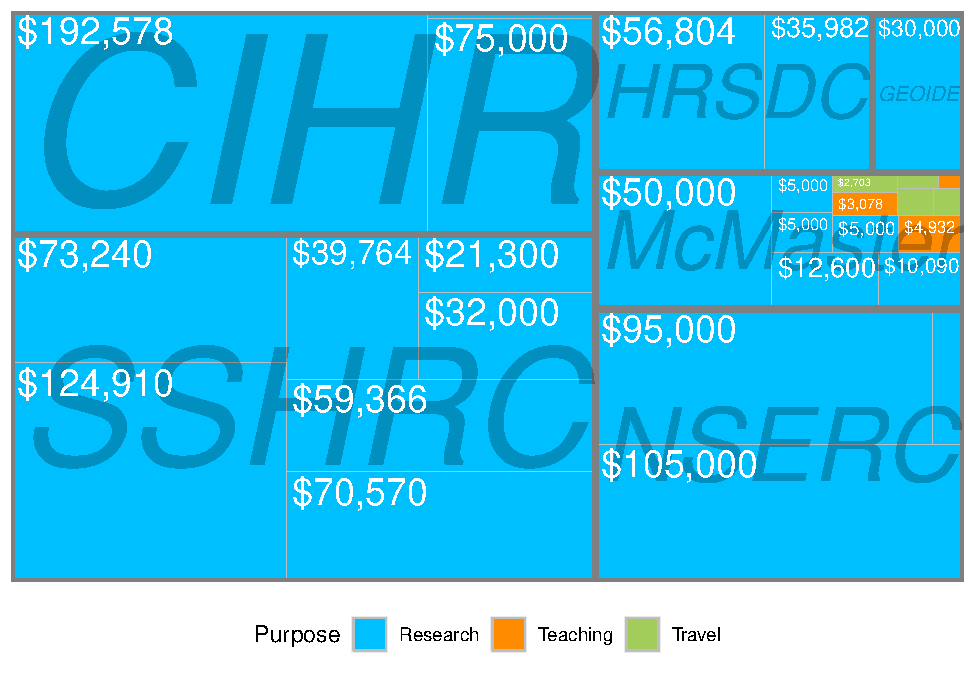
\includegraphics[width=0.7\linewidth]{paez-rcs-cv_files/figure-latex/research-funding-plot-1} 

}

\caption{\label{fig:research-funding-share}My share of research funds by source}\label{fig:research-funding-plot}
\end{figure}

\subsection{Detailed Funding}\label{detailed-funding}

\begin{cventries}
    \cventry{Active sustainable transportation: barriers to cycling among university students}{McMaster University, International Initiatives Micro Fund, Canada}{CAD  5,000}{2024}{\begin{cvitems}
\item PI: Antonio Paez; team size: 2 researchers
\end{cvitems}}
    \cventry{Conference Grant}{Arts and Research Board McMaster University, Canada}{CAD 1,700}{2024}{\begin{cvitems}
\item PI: Antonio Paez; team size: 1 researchers
\end{cvitems}}
    \cventry{Publication and evaluation of the effectiveness of an open-source book to teach spatial statistics}{McPherson Institute-McMaster University Libraries, Canada}{CAD 4,932}{2021-2022}{\begin{cvitems}
\item PI: Antonio Paez; team size: 2 researchers
\end{cvitems}}
    \cventry{Mobilizing Justice}{Social Sciences and Humanities Research Council, Canada}{CAD 2,498,195}{2020-2025}{\begin{cvitems}
\item PI: Steven Farber; team size: 10 researchers
\end{cvitems}}
    \cventry{CHildren's Independent Mobility Environments (CHIME)}{Social Sciences and Humanities Research Council, Canada}{CAD 296,830}{2020-2025}{\begin{cvitems}
\item PI: E. Owen D. Waygood; team size: 4 researchers
\end{cvitems}}
    \cventry{Examining traffic safety challenges of older Pedestrians in Canada}{McMaster Interdisciplinary Research Fund, Canada}{CAD 42,000}{2018-2019}{\begin{cvitems}
\item PI: Antonio Paez; team size: 4 researchers
\end{cvitems}}
    \cventry{Do Closed Schools Mean Disappearing Value? Exploring the Decapitalization of Education in Neighbourhood House Prices in Hamilton}{Social Sciences and Humanities Research Council, Canada}{CAD 49,705}{2017-2018}{\begin{cvitems}
\item PI: Christopher Higgins; team size: 2 researchers
\end{cvitems}}
    \cventry{Technology for Optimal Aging: An exploratory study of the effects of automobile innovations on the lived experience of older drivers, their mobility, and social policy}{Labrage Optimal Aging Initiative, Canada}{CAD 50,449}{2014-2015}{\begin{cvitems}
\item PI: Amanda Grenier; team size: 4 researchers
\end{cvitems}}
    \cventry{Incentive Funding}{McMaster University, Canada}{CAD 5,000}{2014}{\begin{cvitems}
\item PI: Antonio Paez; team size: 1 researchers
\end{cvitems}}
    \cventry{Critical infrastructure: evaluating the effect of network topology and autocorrelation}{Natural Sciences and Engineering Research Council, Canada}{CAD 95,000}{2011-2016}{\begin{cvitems}
\item PI: Antonio Paez; team size: 1 researchers
\end{cvitems}}
    \cventry{Enhancing the Mobility and Health of Older Adults}{Canadian Institutes of Health Research, Canada}{CAD 25,000}{2011}{\begin{cvitems}
\item PI: Heather McKay; team size: 6 researchers
\end{cvitems}}
    \cventry{Walk the Talk: Transforming the Built Environment to Enhance Mobility in Seniors}{Canadian Institutes of Health Research, Canada}{CAD 1,500,000}{2010-2016}{\begin{cvitems}
\item PI: Heather McKay; team size: 10 researchers
\end{cvitems}}
    \cventry{Canada’s Blood Futures: Geography, Demographic Change, and the Supply and Demand of Blood in Canada}{Canadian Institutes of Health Research, Canada}{CAD 240,723}{2010-2013}{\begin{cvitems}
\item PI: Antonio Paez; team size: 4 researchers
\end{cvitems}}
    \cventry{Parks, shops, and friends: how do the built and social environments influence travel behavior?}{Social Sciences and Humanities Research Council, Canada}{CAD 91,550}{2010-2012}{\begin{cvitems}
\item PI: Antonio Paez; team size: 2 researchers
\end{cvitems}}
    \cventry{Conference Grant}{Arts and Research Board McMaster University, Canada}{CAD 1,326}{2010}{\begin{cvitems}
\item PI: Antonio Paez; team size: 1 researchers
\end{cvitems}}
    \cventry{Understanding the transportation situation of Canadian adults with disabilities: Identifying barriers for adults with disabilities who travel locally and long-distance}{Human Resources and Social Development Canada, Canada}{CAD 35,982}{2009}{\begin{cvitems}
\item PI: Antonio Paez; team size: 3 researchers
\end{cvitems}}
    \cventry{Understanding barriers to participation in sport and other physical activities}{Social Sciences and Humanities Research Council, Canada}{CAD 106,500}{2008-2011}{\begin{cvitems}
\item PI: Darren M. Scott; team size: 2 researchers
\end{cvitems}}
    \cventry{Developing a web-based survey to collect student travel behavior information}{Centre for Leadership in Learning McMaster University, Canada}{CAD 800}{2008}{\begin{cvitems}
\item PI: Antonio Paez; team size: 1 researchers
\end{cvitems}}
    \cventry{Travel Grant}{North American Regional Science Council, US}{USD 500}{2008}{\begin{cvitems}
\item PI: Antonio Paez; team size: 1 researchers
\end{cvitems}}
    \cventry{Spatial Mismatch in Canadian Communities: The Socio-economic Outcomes of Transportation Infrastructure and Access}{Human Resources and Social Development Canada, Canada}{CAD 56,804}{2008}{\begin{cvitems}
\item PI: Antonio Paez; team size: 5 researchers
\end{cvitems}}
    \cventry{Blood donor research: Individual determinants and geographical profile of blood donors}{Social Sciences and Humanities Research Council, Canada}{CAD 40,000}{2007-2008}{\begin{cvitems}
\item PI: Antonio Paez; team size: 3 researchers
\end{cvitems}}
    \cventry{Conference Grant}{Arts and Research Board McMaster University, Canada}{CAD 2,045}{2007}{\begin{cvitems}
\item PI: Antonio Paez; team size: 1 researchers
\end{cvitems}}
    \cventry{Social Influence on Travel Behavior: A Case Study of the Decision to Telecommute}{Social Sciences and Humanities Research Council, Canada}{CAD 88,212}{2005-2007}{\begin{cvitems}
\item PI: Antonio Paez; team size: 2 researchers
\end{cvitems}}
    \cventry{International Workshop Frontiers in Transportation: Social and Spatial Interactions}{Natural Sciences and Engineering Research Council, Canada}{CAD 8,660}{2005}{\begin{cvitems}
\item PI: Antonio Paez; team size: 4 researchers
\end{cvitems}}
    \cventry{Conference Grant}{Arts and Research Board McMaster University, Canada}{CAD 2,703}{2005}{\begin{cvitems}
\item PI: Antonio Paez; team size: 1 researchers
\end{cvitems}}
    \cventry{Incentive Funding}{McMaster University, Canada}{CAD 5,000}{2004}{\begin{cvitems}
\item PI: Antonio Paez; team size: 1 researchers
\end{cvitems}}
    \cventry{Using spreadsheets and graphics to improve mathematical intuition in geographical problem solving: The case of Locational Analysis}{Centre for Leadership in Learning McMaster University, Canada}{CAD 3,078}{2004}{\begin{cvitems}
\item PI: Antonio Paez; team size: 1 researchers
\end{cvitems}}
    \cventry{Modeling Continuous-space Contextual Effects in Transportation Systems}{Natural Sciences and Engineering Research Council, Canada}{CAD 105,000}{2003-2007}{\begin{cvitems}
\item PI: Antonio Paez; team size: 1 researchers
\end{cvitems}}
    \cventry{Transportation Implications of Canada's Aging Society}{Geomatics for Informed Decisions (GEOIDE), Canada}{CAD 150,000}{2003-2004}{\begin{cvitems}
\item PI: Darren M. Scott; team size: 6 researchers
\end{cvitems}}
    \cventry{Start-up Funds}{McMaster University, Canada}{CAD 50,000}{2002}{\begin{cvitems}
\item PI: Antonio Paez; team size: 1 researchers
\end{cvitems}}
\end{cventries}

\section{Research Impact}\label{research-impact}

Fig. \ref{fig:citations} gives a summary of my research impact according
to Google Scholar. As of Sep, 2024, my research has been cited a total
of 12,480 times, and my h-index is 57. The i10-index indicates that 130,
or approximately 62\% of my publications have been cited ten times or
more.

The impact of my work can also be appreciated by the breadth of the
fields in which it is cited. According to Web of Science (Fig.
\ref{fig:citations-by-field}), my research is cited by scholars in
numerous disciplines, notably in Transportation, Environmental
Science/Studies, Geography, Economics, and Urban Studies. My
publications have been cited by researchers in more than 100 countries;
as seen in Fig. \ref{fig:citations-by-country}, most citations to my
work are by researchers in the United States, China, Canada, England,
and Spain.

Lastly, my work has contributed to inform research that aligns with the
United Nations Sustainable Development Goals (see Fig.
\ref{fig:citations-by-sdg}), particularly goals 11:Sustainable Cities
And Communities, 03:Good Health And Well Being, 13:Climate Action,
15:Life On Land, and 16:Peace And Justice Strong Institutions.

Combined with the level of funding described above, the cost-effect of
my research is approximately CAD 7,181 per peer-reviewed article (not
counting book chapters, edited books, or books). To put this number in
context, this is equivalent to 54\% of a one-year graduate research
assistantship at my institution. In terms of impact, the cost-effect of
my research is CAD 90 per citation.

\begin{figure}

{\centering \includegraphics[width=0.6\linewidth]{paez-rcs-cv_files/figure-latex/citations-plot-1} 

}

\caption{\label{fig:citations}Citations per year (data from Google Scholar)}\label{fig:citations-plot}
\end{figure}

\begin{figure}

{\centering \includegraphics[width=0.7\linewidth]{paez-rcs-cv_files/figure-latex/citations-field-1} 

}

\caption{\label{fig:citations-by-field}Citations by field (data from Web of Science)}\label{fig:citations-field}
\end{figure}

\begin{figure}

{\centering \includegraphics[width=0.7\linewidth]{paez-rcs-cv_files/figure-latex/citations-country-1} 

}

\caption{\label{fig:citations-by-sdg}Citations by country (data from Web of Science)}\label{fig:citations-country}
\end{figure}

\begin{figure}

{\centering \includegraphics[width=0.7\linewidth]{paez-rcs-cv_files/figure-latex/citations-sdg-1} 

}

\caption{\label{fig:citations-by-country}Citations by Sustainable Development Goal (data from Web of Science)}\label{fig:citations-sdg}
\end{figure}

\section{Research Output}\label{research-output}

It is conventional in my fields of expertise to list authors in order of
their contributions. The first and second authors are credited with
doing a majority of the work. The exception to this general rule is when
the last author is the senior author and has provided, in addition to
other contributions, supervisory support to the rest of the team.

\subsection{At a Glance}\label{at-a-glance}

Table \ref{tab:bibliography-at-a-glance} provides some key information
about my publication record. In addition to the items listed there, I am
co-editor of 3 edited books. Fig. \ref{fig:key-topics} maps the
relationship between key topics in my peer-reviewed publications, based
on keywords of the documents. Fig. \ref{fig:intl-colabs} maps my
international research collaborations.

\begin{table}[H]
\centering
\caption{\label{tab:unnamed-chunk-2}\label{tab:bibliography-at-a-glance}Bibliography at a glance}
\centering
\fontsize{7}{9}\selectfont
\begin{tabular}[t]{l|r|r|r|l|l|l|l|l}
\hline
Type & No. of Items & Mean No. Authors & Max. No. Authors & Single Author & First Author & Second Author & Senior Author & Other Author\\
\hline
Books & 1 & 2.00 & 2 & 0 (0\%) & 1 (100\%) & 0 (0\%) & 0 (0\%) & 0 (0\%)\\
\hline
Book chapters & 9 & 3.00 & 4 & 1 (11\%) & 4 (44\%) & 2 (22.22\%) & 2 (22.22\%) & 0 (0\%)\\
\hline
Peer reviewed articles & 157 & 3.35 & 7 & 12 (8\%) & 34 (22\%) & 61 (39\%) & 31 (20\%) & 19 (12\%)\\
\hline
Peer reviewed conference presentations & 43 & 3.65 & 6 & 2 (5\%) & 10 (23\%) & 19 (44\%) & 4 (9\%) & 8 (19\%)\\
\hline
\end{tabular}
\end{table}

\begin{figure}

{\centering \includegraphics[width=0.7\linewidth]{paez-rcs-cv_files/figure-latex/key-topics-plot-1} 

}

\caption{\label{fig:key-topics}Key topics in my peer-reviewed publications}\label{fig:key-topics-plot}
\end{figure}

\begin{figure}

{\centering \includegraphics[width=0.6\linewidth]{paez-rcs-cv_files/figure-latex/intl-colabs-plot-1} 

}

\caption{\label{fig:intl-colabs}International collaborations}\label{fig:intl-colabs-plot}
\end{figure}

\newpage

\section{Lifetime Publications}\label{lifetime-publications}

\subsection{Books}\label{books}

\phantomsection\label{refs-5cf02433c34c551c872e4694d767b53b}
\begin{CSLReferences}{0}{0}
\bibitem[\citeproctext]{ref-paez2023discrete}
\CSLLeftMargin{1. }%
\CSLRightInline{Páez, A., \& Boisjoly, G. (2023). \emph{Discrete choice
analysis with R}. Springer Cham.
\url{https://doi.org/10.1007/978-3-031-20719-8}}

\end{CSLReferences}

\subsection{Edited Books}\label{edited-books}

\phantomsection\label{refs-4c4fe3a0208d54385a9ff2cba1abdbdb}
\begin{CSLReferences}{0}{0}
\bibitem[\citeproctext]{ref-franklin2018population}
\CSLLeftMargin{1. }%
\CSLRightInline{Franklin, R. S., Leeuwen, E. S. van, \& Páez, A. (2018).
\emph{Population loss: The role of transportation and other issues}.
Academic Press.}

\bibitem[\citeproctext]{ref-delmelle2015spatial}
\CSLLeftMargin{2. }%
\CSLRightInline{Kanaroglou, P., Delmelle, E., \& Páez, A. (2015).
\emph{Spatial analysis in health geography}. Ashgate Publishing, Ltd.}

\bibitem[\citeproctext]{ref-paez2009progress}
\CSLLeftMargin{3. }%
\CSLRightInline{Páez, A., Gallo, J., Buliung, R. N., \& Dall'erba, S.
(2009). \emph{Progress in spatial analysis: Methods and applications}.
Springer Science \& Business Media.}

\end{CSLReferences}

\subsection{Book Chapters}\label{book-chapters}

\phantomsection\label{refs-fa434c1e835439e2e6e79b47ebeff6e2}
\begin{CSLReferences}{0}{0}
\bibitem[\citeproctext]{ref-Barbosa2020}
\CSLLeftMargin{1. }%
\CSLRightInline{Barbosa, E., Féres, J., Haddad, E., \& Páez, A. (2020).
Climate change and land use pattern in brazil. In J.-C. Thill (Ed.),
\emph{Innovations in urban and regional systems: Contributions from
GIS\&t, spatial analysis and location modeling} (pp. 443--472). Springer
International Publishing.
\url{https://doi.org/10.1007/978-3-030-43694-0_20}}

\bibitem[\citeproctext]{ref-Franklin2020transportation}
\CSLLeftMargin{2. }%
\CSLRightInline{Franklin, R. S., Leeuwen, E. S. van, \& Páez, A. (2018).
\emph{Transportation where people leave: An introduction} (Vol. 2, pp.
1--14). \href{https://www.scopus.com}{www.scopus.com}}

\bibitem[\citeproctext]{ref-Paez2020clustering}
\CSLLeftMargin{3. }%
\CSLRightInline{Páez, A., López-Hernández, F. A., Ortega-García, J. A.,
\& Ruiz, M. (2016). \emph{Clustering and co-occurrence of cancer types:
A comparison of techniques with an application to pediatric cancer in
Murcia, Spain} (pp. 47--68).
\href{https://www.scopus.com}{www.scopus.com}}

\bibitem[\citeproctext]{ref-Paez2016access}
\CSLLeftMargin{4. }%
\CSLRightInline{Páez, A. (2016). \emph{Access and social complexity:
Identifying and managing access requirements across social groups and
across the world} (pp. 190--217).
\href{https://www.scopus.com}{www.scopus.com}}

\bibitem[\citeproctext]{ref-Paez2014micro}
\CSLLeftMargin{5. }%
\CSLRightInline{Páez, A., Hernández, F. A. L., Ruiz, M., \& Logan, J.
(2014). \emph{Micro-geography of segregation: Evidence from historical
US census data} (pp. 91--110).
\href{https://www.scopus.com}{www.scopus.com}}

\bibitem[\citeproctext]{ref-Mur2012local}
\CSLLeftMargin{6. }%
\CSLRightInline{Mur, J., \& Páez, A. (2012). \emph{Local weighting
matrices or the necessity of flexibility} (Vol. 75, pp. 193--212).
\href{https://www.scopus.com}{www.scopus.com}}

\bibitem[\citeproctext]{ref-Paez2010progress}
\CSLLeftMargin{7. }%
\CSLRightInline{Páez, A., Le Gallo, J., Buliung, R. N., \& Dall'Erba, S.
(2010). \emph{Progress in spatial analysis: introduction} (Vol. 63, pp.
1--13). \href{https://www.scopus.com}{www.scopus.com}}

\bibitem[\citeproctext]{ref-Farber2010topology}
\CSLLeftMargin{8. }%
\CSLRightInline{Farber, S., Páez, A., \& Volz, E. (2010).
\emph{Topology, dependency tests and estimation bias in network
autoregressive models} (Vol. 63, pp. 29--57).
\href{https://www.scopus.com}{www.scopus.com}}

\bibitem[\citeproctext]{ref-Paez2009gwr}
\CSLLeftMargin{9. }%
\CSLRightInline{Páez, A., \& Wheeler, D. C. (2009). \emph{Geographically
weighted regression} (pp. 407--414).
\href{https://www.scopus.com}{www.scopus.com}}

\end{CSLReferences}

\subsection{Reports}\label{reports}

\phantomsection\label{refs-a73ec60e58689bbc3e562183c5b03f80}
\begin{CSLReferences}{0}{0}
\bibitem[\citeproctext]{ref-MJ-A2-0002}
\CSLLeftMargin{1. }%
\CSLRightInline{Soukhov, A., \& Páez, A. (2024). \emph{Accessibility
analysis for planning applications} (MJ-A2-0002). Mobilizing Justice.
\url{https://github.com/soukhova/MJ-Accessibility-Blogs}}

\bibitem[\citeproctext]{ref-MJ-0001}
\CSLLeftMargin{2. }%
\CSLRightInline{Soukhov, A., Tiznado-Aitken, I., Palm, M., Farber, S.,
\& Páez, A. (2023). \emph{Searching for standards of fairness in the
transportation justice literature} (MJ-0001). Mobilizing Justice.
\url{https://example.com/summarizing-output}}

\bibitem[\citeproctext]{ref-paezDisabilities2010}
\CSLLeftMargin{3. }%
\CSLRightInline{Steven, \& Páez, A. (2010). \emph{Understanding the
transportation situation of canadian adults with disabilities}. Human
Resources; Social Development Canada.
\url{https://www.researchgate.net/profile/Steven-Farber-2/publication/254608932_Participation_and_desire_leisure_activities_among_Canadian_adults_with_disabilities/links/00463528d2c12cafd9000000/Participation-and-desire-leisure-activities-among-Canadian-adults-with-disabilities.pdf}}

\bibitem[\citeproctext]{ref-paezSocial2008}
\CSLLeftMargin{4. }%
\CSLRightInline{Steven, Páez, A., Mercado, R. G., Farber, S., Morency,
C., \& Roorda, M. (2009). \emph{Mobility and social exclusion in
canadian communities: An empirical investigation of opportunity access
and deprivation from the perspective of vulnerable groups}. Human
Resources; Social Development Canada.
\url{https://www.researchgate.net/profile/Catherine-Morency/publication/233997689_Mobility_and_Social_Exclusion_in_Canadian_Communities_An_Empirical_Investigation_of_Opportunity_Access_and_Deprivation/links/54f066980cf25f74d7267b6f/Mobility-and-Social-Exclusion-in-Canadian-Communities-An-Empirical-Investigation-of-Opportunity-Access-and-Deprivation.pdf}}

\end{CSLReferences}

\subsection{Peer-Reviewed Journal Articles
(Published)}\label{peer-reviewed-journal-articles-published}

\phantomsection\label{refs-7f2a2b0ccdb42055bd8a489a90181671}
\begin{CSLReferences}{0}{0}
\bibitem[\citeproctext]{ref-tavakoli_traffic_2024}
\CSLLeftMargin{1. }%
\CSLRightInline{Tavakoli, Z., Abdollahi, S., Waygood, E. O. D., Páez,
A., \& Boisjoly, G. (2024). Traffic danger's potential impact on
children's accessibility. \emph{Transportation Research Part D:
Transport and Environment}, \emph{135}, 104370.
\url{https://doi.org/10.1016/j.trd.2024.104370}}

\bibitem[\citeproctext]{ref-jamal_well-being_2024}
\CSLLeftMargin{2. }%
\CSLRightInline{Jamal, S., \& Paez, A. (2024). Well-being implications
of immobility during COVID-19: Evidence from a student sample in
Bangladesh using the satisfaction with life scale.
\emph{Transportation}, \emph{51}(5), 2019--2049.
\url{https://doi.org/10.1007/s11116-023-10395-z}}

\bibitem[\citeproctext]{ref-rey-blanco_geo-referenced_2024}
\CSLLeftMargin{3. }%
\CSLRightInline{Rey-Blanco, D., Arbues, P., Lopez, F., \& Paez, A.
(2024). A geo-referenced micro-data set of real estate listings for
Spain's three largest cities. \emph{Environment and Planning B: Urban
Analytics and City Science}, \emph{51}(6), 1369--1379.
\url{https://doi.org/10.1177/23998083241242844}}

\bibitem[\citeproctext]{ref-desjardinsFramingActive2024}
\CSLLeftMargin{4. }%
\CSLRightInline{Desjardins, E., Lam, J., Reynard, D., Collins, D.,
Waygood, E. O. D., \& Páez, A. (2024). Framing active school travel in
Ontario, or how spinach is good for you. \emph{Transportation Research
Part A: Policy and Practice}, \emph{180}, 103953.
\url{https://doi.org/10.1016/j.tra.2024.103953}}

\bibitem[\citeproctext]{ref-soukhovMultimodalSpatial2024}
\CSLLeftMargin{5. }%
\CSLRightInline{Soukhov, A., Tarriño-Ortiz, J., Soria-Lara, J. A., \&
Páez, A. (2024). Multimodal spatial availability: A singly-constrained
measure of accessibility considering multiple modes. \emph{PLOS ONE},
\emph{19}(2), e0299077.
\url{https://doi.org/10.1371/journal.pone.0299077}}

\bibitem[\citeproctext]{ref-rey-blanco2024UsingMachine}
\CSLLeftMargin{6. }%
\CSLRightInline{Rey-Blanco, D., Arbués, P., López, F. A., \& Páez, A.
(2024). Using machine learning to identify spatial market segments. A
reproducible study of major Spanish markets. \emph{Environment and
Planning B: Urban Analytics and City Science}, \emph{51}(1), 89--108.
\url{https://doi.org/10.1177/23998083231166952}}

\bibitem[\citeproctext]{ref-merrall2024school}
\CSLLeftMargin{7. }%
\CSLRightInline{Merrall, J., Higgins, C. D., \& Páez, A. (2024). What's
a school worth to a neighborhood? A spatial hedonic analysis of property
prices in the context of accommodation reviews in ontario.
\emph{Geographical Analysis}, \emph{56}(2), 217--243.
https://doi.org/\url{https://doi.org/10.1111/gean.12377}}

\bibitem[\citeproctext]{ref-JAMAL2024100130}
\CSLLeftMargin{8. }%
\CSLRightInline{Jamal, S., \& Páez, A. (2024). Exploring modal shift in
non-active sustainable transport modes during the first wave of COVID-19
in bangladesh. \emph{Multimodal Transportation}, \emph{3}(2), 100130.
https://doi.org/\url{https://doi.org/10.1016/j.multra.2024.100130}}

\bibitem[\citeproctext]{ref-jamal2024socioeconomic}
\CSLLeftMargin{9. }%
\CSLRightInline{Jamal, S., \& Páez, A. (2024). Socio-economic and
demographic differences in the impact of COVID-19 on personal travel in
the Global South. \emph{Transport Reviews}, \emph{44}(2), 272--298.
\url{https://doi.org/10.1080/01441647.2023.2295377}}

\bibitem[\citeproctext]{ref-soukhov2023introducing}
\CSLLeftMargin{10. }%
\CSLRightInline{Soukhov, A., Páez, A., Higgins, C. D., \& Mohamed, M.
(2023). Introducing spatial availability, a singly-constrained measure
of competitive accessibility {[}Journal Article{]}. \emph{PLOS ONE},
\emph{18}(1), e0278468.
\url{https://doi.org/10.1371/journal.pone.0278468}}

\bibitem[\citeproctext]{ref-RN7294}
\CSLLeftMargin{11. }%
\CSLRightInline{Soukhov, A., \& Páez, A. (2023). TTS2016R: A data set to
study population and employment patterns from the 2016 Transportation
Tomorrow Survey in the Greater Golden Horseshoe Area, Ontario, Canada
{[}Journal Article{]}. \emph{Environment and Planning B: Urban Analytics
and City Science}, \emph{50}(2), 556--563.
\url{https://doi.org/10.1177/23998083221146781}}

\bibitem[\citeproctext]{ref-RN7454}
\CSLLeftMargin{12. }%
\CSLRightInline{Santos, B. D. dos dos, Ribeiro, R. M., Páez, A., Kampel,
M., Pinho, C. M. D. de, \& Amaral, S. (2023). State-of-the-art and
framework for identifying urban patterns by remote sensing data
{[}Journal Article{]}. \emph{Revista Brasileira de Cartografia},
\emph{75}. \url{https://doi.org/10.14393/rbcv75n0a-67966}}

\bibitem[\citeproctext]{ref-RN7347}
\CSLLeftMargin{13. }%
\CSLRightInline{Santos, B. D. dos, Pinho, C. M. D. de, Páez, A., \&
Amaral, S. (2023). Identifying urban and socio-environmental patterns of
Brazilian Amazonian cities by remote sensing and machine learning
{[}Journal Article{]}. \emph{Remote Sensing}, \emph{15}(12), 3102.
\url{https://www.mdpi.com/2072-4292/15/12/3102}}

\bibitem[\citeproctext]{ref-cheng2023mobility}
\CSLLeftMargin{14. }%
\CSLRightInline{Cheng, L., Wang, J., \& Páez, A. (2023). Mobility of
older adults and the living environment: introduction {[}Journal
Article{]}. \emph{Journal of Transport Geography}, \emph{106}, 103525.
https://doi.org/\url{https://doi.org/10.1016/j.jtrangeo.2022.103525}}

\bibitem[\citeproctext]{ref-brum2023}
\CSLLeftMargin{15. }%
\CSLRightInline{Brum-Bastos, V., \& Páez, A. (2023). Hägerstrand meets
big data: Time-geography in the age of mobility analytics {[}Journal
Article{]}. \emph{Journal of Geographical Systems}, \emph{25}(3),
327--336. \url{https://doi.org/10.1007/s10109-023-00421-0}}

\bibitem[\citeproctext]{ref-whalen2022reliability}
\CSLLeftMargin{16. }%
\CSLRightInline{Whalen, K., \& Páez, A. (2022). Reliability of the
reflective learning framework for assessing higher-order thinking in
geography and sustainability courses {[}Journal Article{]}.
\emph{Journal of Geography}, \emph{121}(1), 18--33.
\url{https://doi.org/10.1080/00221341.2021.2003848}}

\bibitem[\citeproctext]{ref-RN6494}
\CSLLeftMargin{17. }%
\CSLRightInline{Sears, S., Moataz, M., Ferguson, M., Razavi, S., \&
Páez, A. (2022). Perceived barriers to the movement of goods in Canada:
A grounded theory investigation {[}Journal Article{]}.
\emph{Transportation Research Part A: Policy and Practice}, \emph{162},
27--45. \url{https://doi.org/10.1016/j.tra.2022.05.011}}

\bibitem[\citeproctext]{ref-RN7077}
\CSLLeftMargin{18. }%
\CSLRightInline{Páez, A. (2022). Reproducibility of research during
COVID‐19: Examining the case of population density and the basic
reproductive rate from the perspective of spatial analysis {[}Journal
Article{]}. \emph{Geographical Analysis}, \emph{54}(4), 860--880.
\url{https://doi.org/10.1111/gean.12307}}

\bibitem[\citeproctext]{ref-RN7075}
\CSLLeftMargin{19. }%
\CSLRightInline{Desjardins, E., Tavakoli, Z., Páez, A., \& Waygood, E.
O. (2022). Children's access to non-school destinations by active or
independent travel: A scoping review. In \emph{International Journal of
Environmental Research and Public Health} (Electronic Article No. 19;
Vol. 19). \url{https://doi.org/10.3390/ijerph191912345}}

\bibitem[\citeproctext]{ref-RN6502}
\CSLLeftMargin{20. }%
\CSLRightInline{Desjardins, E., Higgins, C. D., Scott, D. M., Apatu, E.,
\& Páez, A. (2022). Correlates of bicycling trip flows in hamilton,
Ontario: Fastest, quietest, or balanced routes? {[}Journal Article{]}.
\emph{Transportation}, \emph{49}(3), 867--895.
\url{https://doi.org/10.1007/s11116-021-10197-1}}

\bibitem[\citeproctext]{ref-desjardins2022examining}
\CSLLeftMargin{21. }%
\CSLRightInline{Desjardins, E., Higgins, C. D., \& Páez, A. (2022).
Examining equity in accessibility to bike share: A balanced floating
catchment area approach. \emph{Transportation Research Part D: Transport
and Environment}, \emph{102}, 103091.
https://doi.org/\url{https://doi.org/10.1016/j.trd.2021.103091}}

\bibitem[\citeproctext]{ref-demitiry2022accessibility}
\CSLLeftMargin{22. }%
\CSLRightInline{Demitiry, M., Higgins, C. D., Páez, A., \& Miller, E. J.
(2022). Accessibility to primary care physicians: Comparing floating
catchments with a utility-based approach. \emph{Journal of Transport
Geography}, \emph{101}, 103356.
\url{https://doi.org/10.1016/j.jtrangeo.2022.103356}}

\bibitem[\citeproctext]{ref-brown2022spatial}
\CSLLeftMargin{23. }%
\CSLRightInline{Brown, M. J., Scott, D. M., \& Páez, A. (2022). A
spatial modeling approach to estimating bike share traffic volume from
GPS data {[}Journal Article{]}. \emph{Sustainable Cities and Society},
\emph{76}, 103401. \url{https://doi.org/10.1016/j.scs.2021.103401}}

\bibitem[\citeproctext]{ref-whalen2021student}
\CSLLeftMargin{24. }%
\CSLRightInline{Whalen, K., \& Páez, A. (2021). Student perceptions of
reflection and the acquisition of higher-order thinking skills in a
university sustainability course {[}Journal Article{]}. \emph{Journal of
Geography in Higher Education}, \emph{45}(1), 108--127.
\url{https://doi.org/10.1080/03098265.2020.1804843}}

\bibitem[\citeproctext]{ref-RN6374}
\CSLLeftMargin{25. }%
\CSLRightInline{Páez, A., Lopez, F. A., Menezes, T., Cavalcanti, R., \&
Rocha Pitta, M. G. da. (2021). A spatio-temporal analysis of the
environmental correlates of COVID-19 incidence in Spain {[}Journal
Article{]}. \emph{Geographical Analysis}, \emph{53}(3), 397--421.
\url{https://doi.org/10.1111/gean.12241}}

\bibitem[\citeproctext]{ref-paez2021examination}
\CSLLeftMargin{26. }%
\CSLRightInline{Páez, A., \& Higgins, C. D. (2021). An examination of
the accessibility implications of a pilot COVID-19 vaccination program
in Hamilton, Ontario {[}Journal Article{]}. \emph{Findings}.
\url{https://doi.org/10.32866/001c.24082}}

\bibitem[\citeproctext]{ref-RN6283}
\CSLLeftMargin{27. }%
\CSLRightInline{Páez, A. (2021). Open spatial sciences: An introduction
{[}Journal Article{]}. \emph{Journal of Geographical Systems},
\emph{23}(4), 467--476.
\url{https://doi.org/10.1007/s10109-021-00364-4}}

\bibitem[\citeproctext]{ref-RN6395}
\CSLLeftMargin{28. }%
\CSLRightInline{Pereira, R. H. M., Braga, C. K. V., Servo, L. M., Serra,
B., Amaral, P., Gouveia, N., \& Páez, A. (2021). Geographic access to
COVID-19 healthcare in Brazil using a balanced float catchment area
approach {[}Journal Article{]}. \emph{Social Science \& Medicine},
\emph{273}. \url{https://doi.org/10.1016/j.socscimed.2021.113773}}

\bibitem[\citeproctext]{ref-RN6362}
\CSLLeftMargin{29. }%
\CSLRightInline{Lira, B. M., \& Páez, A. (2021). Do drivers dream of
walking? An investigation of travel mode dissonance from the perspective
of affective values {[}Journal Article{]}. \emph{Journal of Transport \&
Health}, \emph{20}. \url{https://doi.org/10.1016/j.jth.2021.101015}}

\bibitem[\citeproctext]{ref-RN6396}
\CSLLeftMargin{30. }%
\CSLRightInline{Higgins, C. D., Páez, A., Kim, G., \& Wang, J. (2021).
Changes in accessibility to emergency and community food services during
COVID-19 and implications for low income populations in Hamilton,
Ontario {[}Journal Article{]}. \emph{Social Science \& Medicine},
\emph{291}. \url{https://doi.org/10.1016/j.socscimed.2021.114442}}

\bibitem[\citeproctext]{ref-RN6278}
\CSLLeftMargin{31. }%
\CSLRightInline{Eldeeb, G., Mohamed, M., \& Páez, A. (2021). Built for
active travel? Investigating the contextual effects of the built
environment on transportation mode choice {[}Journal Article{]}.
\emph{Journal of Transport Geography}, \emph{96}.
\url{https://doi.org/10.1016/j.jtrangeo.2021.103158}}

\bibitem[\citeproctext]{ref-RN6358}
\CSLLeftMargin{32. }%
\CSLRightInline{Doulabi, S., Hassan, H. M., Ferguson, M. R., Razavi, S.,
\& Páez, A. (2021). Exploring the determinants of older adults'
susceptibility to pedestrians' incidents {[}Journal Article{]}.
\emph{Accident Analysis and Prevention}, \emph{155}.
\url{https://doi.org/10.1016/j.aap.2021.106100}}

\bibitem[\citeproctext]{ref-RN6340}
\CSLLeftMargin{33. }%
\CSLRightInline{Desjardins, E., Higgins, C. D., Scott, D. M., Apatu, E.,
\& Páez, A. (2021). Using environmental audits and photo-journeys to
compare objective attributes and bicyclists' perceptions of bicycle
routes {[}Journal Article{]}. \emph{Journal of Transport \& Health},
\emph{22}. \url{https://doi.org/10.1016/j.jth.2021.101092}}

\bibitem[\citeproctext]{ref-RN6339}
\CSLLeftMargin{34. }%
\CSLRightInline{Desjardins, E., Apatu, E., Razavi, S. D., Higgins, C.
D., Scott, D. M., \& Páez, A. (2021). {``Going through a little bit of
growing pains''}: A qualitative study of the factors that influence the
route choice of regular bicyclists in a developing cycling city
{[}Journal Article{]}. \emph{Transportation Research Part F-Traffic
Psychology and Behaviour}, \emph{81}, 431--444.
\url{https://doi.org/10.1016/j.trf.2021.06.005}}

\bibitem[\citeproctext]{ref-dearruda2021effect}
\CSLLeftMargin{35. }%
\CSLRightInline{de Arruda, R. G., de Menezes, T. A., dos Santos, J. M.
A., Páez, A., \& Lopes, F. (2021). The effect of politician denialist
approach on COVID-19 cases and deaths {[}Journal Article{]}.
\emph{EconomiA}, \emph{22}(3), 214--224.
\url{https://doi.org/10.1016/j.econ.2021.11.007}}

\bibitem[\citeproctext]{ref-RN6353}
\CSLLeftMargin{36. }%
\CSLRightInline{Victoriano, R., Páez, A., \& Carrasco, J.-A. (2020).
Time, space, money, and social interaction: Using machine learning to
classify people's mobility strategies through four key dimensions
{[}Journal Article{]}. \emph{Travel Behaviour and Society}, \emph{20},
1--11. \url{https://doi.org/10.1016/j.tbs.2020.02.004}}

\bibitem[\citeproctext]{ref-RN6366}
\CSLLeftMargin{37. }%
\CSLRightInline{Sarlas, G., Páez, A., \& Axhausen, K. W. (2020).
Betweenness-accessibility: Estimating impacts of accessibility on
networks {[}Journal Article{]}. \emph{Journal of Transport Geography},
\emph{84}. \url{https://doi.org/10.1016/j.jtrangeo.2020.102680}}

\bibitem[\citeproctext]{ref-RN6361}
\CSLLeftMargin{38. }%
\CSLRightInline{Romero, F., Gomez, J., Páez, A., \& Manuel Vassallo, J.
(2020). Toll roads vs.~Public transportation: A study on the acceptance
of congestion-calming measures in Madrid {[}Journal Article{]}.
\emph{Transportation Research Part a-Policy and Practice}, \emph{142},
319--342. \url{https://doi.org/10.1016/j.tra.2020.11.001}}

\bibitem[\citeproctext]{ref-RN6335}
\CSLLeftMargin{39. }%
\CSLRightInline{Páez, A., Hassan, H., Ferguson, M., \& Razavi, S.
(2020). A systematic assessment of the use of opponent variables, data
subsetting and hierarchical specification in two-party crash severity
analysis {[}Journal Article{]}. \emph{Accident Analysis and Prevention},
\emph{144}. \url{https://doi.org/10.1016/j.aap.2020.105666}}

\bibitem[\citeproctext]{ref-RN6346}
\CSLLeftMargin{40. }%
\CSLRightInline{Páez, A., Anjum, Z., Dickson-Anderson, S. E.,
Schuster-Wallace, C. J., Martin Ramos, B., \& Higgins, C. D. (2020).
Comparing distance, time, and metabolic energy cost functions for
walking accessibility in infrastructure-poor regions {[}Journal
Article{]}. \emph{Journal of Transport Geography}, \emph{82}.
\url{https://doi.org/10.1016/j.jtrangeo.2019.102564}}

\bibitem[\citeproctext]{ref-paez2020using}
\CSLLeftMargin{41. }%
\CSLRightInline{Páez, A. (2020). Using Google Community Mobility Reports
to investigate the growth of COVID-19 in the United States {[}Journal
Article{]}. \emph{Findings}. \url{https://doi.org/10.32866/001c.12976}}

\bibitem[\citeproctext]{ref-jamal2020changes}
\CSLLeftMargin{42. }%
\CSLRightInline{Jamal, S., \& Páez, A. (2020). Changes in trip-making
frequency by mode during the COVID-19 emergency in Bangladesh {[}Journal
Article{]}. \emph{Findings}. \url{https://doi.org/10.32866/001c.17977}}

\bibitem[\citeproctext]{ref-RN6364}
\CSLLeftMargin{43. }%
\CSLRightInline{Jamal, S., Mohiuddin, H., \& Páez, A. (2020). How do the
perceptions of neighborhood conditions impact active transportation? A
study in Rajshahi, Bangladesh {[}Journal Article{]}.
\emph{Transportation Research Part D-Transport and Environment},
\emph{87}. \url{https://doi.org/10.1016/j.trd.2020.102525}}

\bibitem[\citeproctext]{ref-RN6382}
\CSLLeftMargin{44. }%
\CSLRightInline{He, L., Páez, A., Jiao, J., An, P., Lu, C., Mao, W., \&
Long, D. (2020). Ambient population and larceny-theft: A spatial
analysis using mobile phone data {[}Journal Article{]}. \emph{Isprs
International Journal of Geo-Information}, \emph{9}(6).
\url{https://doi.org/10.3390/ijgi9060342}}

\bibitem[\citeproctext]{ref-RN6384}
\CSLLeftMargin{45. }%
\CSLRightInline{Cupido, K., Jevtic, P., \& Páez, A. (2020). Spatial
patterns of mortality in the United States: A spatial filtering approach
{[}Journal Article{]}. \emph{Insurance Mathematics \& Economics},
\emph{95}, 28--38.
\url{https://doi.org/10.1016/j.insmatheco.2020.08.003}}

\bibitem[\citeproctext]{ref-RN6282}
\CSLLeftMargin{46. }%
\CSLRightInline{Whalen, K., \& Páez, A. (2019). Development of a new
framework to guide, assess, and evaluate student reflections in a
university sustainability course {[}Journal Article{]}. \emph{Teaching
\& Learning Inquiry-the Issotl Journal}, \emph{7}(1), 55--77.
\url{https://doi.org/10.20343/teachlearninqu.7.1.5}}

\bibitem[\citeproctext]{ref-RN6334}
\CSLLeftMargin{47. }%
\CSLRightInline{Páez, A., Lopez, F., Ruiz, M., \& Camacho, M. (2019).
Inducing non-orthogonal and non-linear decision boundaries in decision
trees via interactive basis functions {[}Journal Article{]}.
\emph{Expert Systems with Applications}, \emph{122}, 183--206.
\url{https://doi.org/10.1016/j.eswa.2018.12.041}}

\bibitem[\citeproctext]{ref-RN6369}
\CSLLeftMargin{48. }%
\CSLRightInline{Páez, A., Higgins, C. D., \& Vivona, S. F. (2019).
Demand and level of service inflation in floating catchment area (FCA)
methods {[}Journal Article{]}. \emph{Plos One}, \emph{14}(6).
\url{https://doi.org/10.1371/journal.pone.0218773}}

\bibitem[\citeproctext]{ref-RN6327}
\CSLLeftMargin{49. }%
\CSLRightInline{Páez, A. (2019). Using spatial filters and exploratory
data analysis to enhance regression models of spatial data {[}Journal
Article{]}. \emph{Geographical Analysis}, \emph{51}(3), 314--338.
\url{https://doi.org/10.1111/gean.12180}}

\bibitem[\citeproctext]{ref-RN6388}
\CSLLeftMargin{50. }%
\CSLRightInline{Martin, B., \& Páez, A. (2019). Individual and
geographic variations in the propensity to travel by active modes in
Vitoria-Gasteiz, Spain {[}Journal Article{]}. \emph{Journal of Transport
Geography}, \emph{76}, 103--113.
\url{https://doi.org/10.1016/j.jtrangeo.2019.03.005}}

\bibitem[\citeproctext]{ref-RN6385}
\CSLLeftMargin{51. }%
\CSLRightInline{Arranz-Lopez, A., Soria-Lara, J. A., Witlox, F., \&
Páez, A. (2019). Measuring relative non-motorized accessibility to
retail activities {[}Journal Article{]}. \emph{International Journal of
Sustainable Transportation}, \emph{13}(9), 639--651.
\url{https://doi.org/10.1080/15568318.2018.1498563}}

\bibitem[\citeproctext]{ref-RN6377}
\CSLLeftMargin{52. }%
\CSLRightInline{Lopez, F. A., Páez, A., Carrasco, J. A., \& Ruminot, N.
A. (2017). Vulnerability of nodes under controlled network topology and
flow autocorrelation conditions {[}Journal Article{]}. \emph{Journal of
Transport Geography}, \emph{59}, 77--87.
\url{https://doi.org/10.1016/j.jtrangeo.2017.02.002}}

\bibitem[\citeproctext]{ref-RN6325}
\CSLLeftMargin{53. }%
\CSLRightInline{Lopez, F. A., \& Páez, A. (2017). Spatial clustering of
high-tech manufacturing and knowledge-intensive service firms in the
Greater Toronto Area {[}Journal Article{]}. \emph{Canadian
Geographer-Geographe Canadien}, \emph{61}(2), 240--252.
\url{https://doi.org/10.1111/cag.12326}}

\bibitem[\citeproctext]{ref-RN6380}
\CSLLeftMargin{54. }%
\CSLRightInline{He, L., Páez, A., \& Liu, D. (2017). Built environment
and violent crime: An environmental audit approach using Google Street
View {[}Journal Article{]}. \emph{Computers Environment and Urban
Systems}, \emph{66}, 83--95.
\url{https://doi.org/10.1016/j.compenvurbsys.2017.08.001}}

\bibitem[\citeproctext]{ref-RN6360}
\CSLLeftMargin{55. }%
\CSLRightInline{He, L., Páez, A., \& Liu, D. (2017). Persistence of
crime hot spots: An ordered probit analysis {[}Journal Article{]}.
\emph{Geographical Analysis}, \emph{49}(1), 3--22.
\url{https://doi.org/10.1111/gean.12107}}

\bibitem[\citeproctext]{ref-RN6391}
\CSLLeftMargin{56. }%
\CSLRightInline{Rojas, C., Páez, A., Barbosa, O., \& Carrasco, J.
(2016). Accessibility to urban green spaces in Chilean cities using
adaptive thresholds {[}Journal Article{]}. \emph{Journal of Transport
Geography}, \emph{57}, 227--240.
\url{https://doi.org/10.1016/j.jtrangeo.2016.10.012}}

\bibitem[\citeproctext]{ref-RN6367}
\CSLLeftMargin{57. }%
\CSLRightInline{Moniruzzaman, M., \& Páez, A. (2016). An investigation
of the attributes of walkable environments from the perspective of
seniors in Montreal {[}Journal Article{]}. \emph{Journal of Transport
Geography}, \emph{51}, 85--96.
\url{https://doi.org/10.1016/j.jtrangeo.2015.12.001}}

\bibitem[\citeproctext]{ref-RN6387}
\CSLLeftMargin{58. }%
\CSLRightInline{Lopez, F. A., Matilla-Garcia, M., Mur, J., Páez, A., \&
Ruiz, M. (2016). A note on the SG(m) test {[}Journal Article{]}.
\emph{Journal of Geographical Systems}, \emph{18}(1), 87--96.
\url{https://doi.org/10.1007/s10109-015-0221-7}}

\bibitem[\citeproctext]{ref-RN6277}
\CSLLeftMargin{59. }%
\CSLRightInline{Roofigari-Esfahan, N., Páez, A., \& Razavi, S. N.
(2015). Location-aware scheduling and control of linear projects:
Introducing space-time float prisms {[}Journal Article{]}. \emph{Journal
of Construction Engineering and Management}, \emph{141}(1).
\url{https://doi.org/10.1061/(asce)co.1943-7862.0000916}}

\bibitem[\citeproctext]{ref-RN6316}
\CSLLeftMargin{60. }%
\CSLRightInline{Neto, R. S., Duarte, G., \& Páez, A. (2015). Gender and
commuting time in Sao Paulo Metropolitan Region {[}Journal Article{]}.
\emph{Urban Studies}, \emph{52}(2), 298--313.
\url{https://doi.org/10.1177/0042098014528392}}

\bibitem[\citeproctext]{ref-RN6326}
\CSLLeftMargin{61. }%
\CSLRightInline{Moniruzzaman, M., Páez, A., Scott, D., \& Morency, C.
(2015). Trip generation of seniors and the geography of walking in
Montreal {[}Journal Article{]}. \emph{Environment and Planning a-Economy
and Space}, \emph{47}(4), 957--976.
\url{https://doi.org/10.1068/a130070p}}

\bibitem[\citeproctext]{ref-RN6394}
\CSLLeftMargin{62. }%
\CSLRightInline{Moniruzzaman, M., Chudyk, A., Páez, A., Winters, M.,
Sims-Gould, J., \& McKay, H. (2015). Travel behavior of low income older
adults and implementation of an accessibility calculator {[}Journal
Article{]}. \emph{Journal of Transport \& Health}, \emph{2}(2),
257--268. \url{https://doi.org/10.1016/j.jth.2015.02.006}}

\bibitem[\citeproctext]{ref-RN6331}
\CSLLeftMargin{63. }%
\CSLRightInline{He, L., Páez, A., Liu, D., \& Jiang, S. (2015). Temporal
stability of model parameters in crime rate analysis: An empirical
examination {[}Journal Article{]}. \emph{Applied Geography}, \emph{58},
141--152. \url{https://doi.org/10.1016/j.apgeog.2015.02.002}}

\bibitem[\citeproctext]{ref-RN6352}
\CSLLeftMargin{64. }%
\CSLRightInline{Goetzke, F., Gerike, R., Páez, A., \& Dugundji, E.
(2015). Social interactions in transportation: Analyzing groups and
spatial networks {[}Journal Article{]}. \emph{Transportation},
\emph{42}(5), 723--731. \url{https://doi.org/10.1007/s11116-015-9643-9}}

\bibitem[\citeproctext]{ref-RN6383}
\CSLLeftMargin{65. }%
\CSLRightInline{Farber, S., Ruiz Marin, M., \& Páez, A. (2015). Testing
for spatial independence using similarity relations {[}Journal
Article{]}. \emph{Geographical Analysis}, \emph{47}(2), 97--120.
\url{https://doi.org/10.1111/gean.12044}}

\bibitem[\citeproctext]{ref-RN6393}
\CSLLeftMargin{66. }%
\CSLRightInline{Wheeler, D. C., Páez, A., Spinney, J., \& Waller, L. A.
(2014). A bayesian approach to hedonic price analysis {[}Journal
Article{]}. \emph{Papers in Regional Science}, \emph{93}(3), 663--683.
\url{https://doi.org/10.1111/pirs.12003}}

\bibitem[\citeproctext]{ref-RN6293}
\CSLLeftMargin{67. }%
\CSLRightInline{Reyes, M., Páez, A., \& Morency, C. (2014). Walking
accessibility to urban parks by children: A case study of Montreal
{[}Journal Article{]}. \emph{Landscape and Urban Planning}, \emph{125},
38--47. \url{https://doi.org/10.1016/j.landurbplan.2014.02.002}}

\bibitem[\citeproctext]{ref-RN6373}
\CSLLeftMargin{68. }%
\CSLRightInline{Pouliou, T., Elliott, S. J., Páez, A., \& Newbold, K. B.
(2014). Building obesity in Canada: Understanding the individual-and
neighbourhood-level determinants using a multi-level approach {[}Journal
Article{]}. \emph{Geospatial Health}, \emph{9}(1), 45--55.
\url{https://doi.org/10.4081/gh.2014.5}}

\bibitem[\citeproctext]{ref-RN6311}
\CSLLeftMargin{69. }%
\CSLRightInline{Moniruzzaman, M., Páez, A., \& Morency, C. (2014).
Compliance potential mapping: A tool to assess potential contributions
of walking towards physical activity guidelines {[}Journal Article{]}.
\emph{Bmc Public Health}, \emph{14}.
\url{https://doi.org/10.1186/1471-2458-14-511}}

\bibitem[\citeproctext]{ref-RN6392}
\CSLLeftMargin{70. }%
\CSLRightInline{Farber, S., Bartholomew, K., Li, X., Páez, A., \& Habib,
K. M. N. (2014). Assessing social equity in distance based transit fares
using a model of travel behavior {[}Journal Article{]}.
\emph{Transportation Research Part a-Policy and Practice}, \emph{67},
291--303. \url{https://doi.org/10.1016/j.tra.2014.07.013}}

\bibitem[\citeproctext]{ref-RN6310}
\CSLLeftMargin{71. }%
\CSLRightInline{Whalen, K. E., Páez, A., \& Carrasco, J. A. (2013). Mode
choice of university students commuting to school and the role of active
travel {[}Journal Article{]}. \emph{Journal of Transport Geography},
\emph{31}, 132--142.
\url{https://doi.org/10.1016/j.jtrangeo.2013.06.008}}

\bibitem[\citeproctext]{ref-da2013isolamento}
\CSLLeftMargin{72. }%
\CSLRightInline{Silva, R. R. da, \& Páez, A. (2013). O isolamento
geoeconômico dos municípios da região norte do brasil: Uma proposta para
quantificá-lo. \emph{Revista Brasileira de Estudos Regionais e Urbanos},
\emph{7}(1), 1--18.}

\bibitem[\citeproctext]{ref-RN6272}
\CSLLeftMargin{73. }%
\CSLRightInline{Scott, D. M., Dugundji, E. R., \& Páez, A. (2013). The
social dimension of activity, travel and location choice behavior
{[}Journal Article{]}. \emph{Journal of Transport Geography}, \emph{31},
212--215. \url{https://doi.org/10.1016/j.jtrangeo.2013.06.009}}

\bibitem[\citeproctext]{ref-RN6323}
\CSLLeftMargin{74. }%
\CSLRightInline{Páez, A., Moniruzzaman, M., Bourbonnais, P.-L., \&
Morency, C. (2013). Developing a web-based accessibility calculator
prototype for the Greater Montreal Area {[}Journal Article{]}.
\emph{Transportation Research Part a-Policy and Practice}, \emph{58},
103--115. \url{https://doi.org/10.1016/j.tra.2013.10.020}}

\bibitem[\citeproctext]{ref-RN6343}
\CSLLeftMargin{75. }%
\CSLRightInline{Páez, A., Lopez, F. A., Ruiz, M., \& Morency, C. (2013).
Development of an indicator to assess the spatial fit of discrete choice
models {[}Journal Article{]}. \emph{Transportation Research Part
B-Methodological}, \emph{56}, 217--233.
\url{https://doi.org/10.1016/j.trb.2013.08.009}}

\bibitem[\citeproctext]{ref-RN6365}
\CSLLeftMargin{76. }%
\CSLRightInline{Páez, A., Farber, S., Mercado, R., Roorda, M., \&
Morency, C. (2013). Jobs and the single parent: An analysis of
accessibility to employment in Toronto {[}Journal Article{]}.
\emph{Urban Geography}, \emph{34}(6), 815--842.
\url{https://doi.org/10.1080/02723638.2013.778600}}

\bibitem[\citeproctext]{ref-RN6299}
\CSLLeftMargin{77. }%
\CSLRightInline{Páez, A., Esita, J., Newbold, K. B., Heddle, N. M., \&
Blake, J. T. (2013). Exploring resource allocation and alternate clinic
accessibility landscapes for improved blood donor turnout {[}Journal
Article{]}. \emph{Applied Geography}, \emph{45}, 89--97.
\url{https://doi.org/10.1016/j.apgeog.2013.08.008}}

\bibitem[\citeproctext]{ref-RN6289}
\CSLLeftMargin{78. }%
\CSLRightInline{Páez, A. (2013). Mapping travelers' attitudes: Does
space matter? {[}Journal Article{]}. \emph{Journal of Transport
Geography}, \emph{26}, 117--125.
\url{https://doi.org/10.1016/j.jtrangeo.2012.09.002}}

\bibitem[\citeproctext]{ref-RN6345}
\CSLLeftMargin{79. }%
\CSLRightInline{Moniruzzaman, M., Páez, A., Habib, K. M. N., \& Morency,
C. (2013). Mode use and trip length of seniors in Montreal {[}Journal
Article{]}. \emph{Journal of Transport Geography}, \emph{30}, 89--99.
\url{https://doi.org/10.1016/j.jtrangeo.2013.03.007}}

\bibitem[\citeproctext]{ref-RN6363}
\CSLLeftMargin{80. }%
\CSLRightInline{Le Gallo, J., \& Páez, A. (2013). Using synthetic
variables in instrumental variable estimation of spatial series models
{[}Journal Article{]}. \emph{Environment and Planning a-Economy and
Space}, \emph{45}(9), 2227--2242. \url{https://doi.org/10.1068/a45443}}

\bibitem[\citeproctext]{ref-RN6312}
\CSLLeftMargin{81. }%
\CSLRightInline{Lavery, T. A., Páez, A., \& Kanaroglou, P. S. (2013).
Driving out of choices: An investigation of transport modality in a
university sample {[}Journal Article{]}. \emph{Transportation Research
Part a-Policy and Practice}, \emph{57}, 37--46.
\url{https://doi.org/10.1016/j.tra.2013.09.010}}

\bibitem[\citeproctext]{ref-RN6319}
\CSLLeftMargin{82. }%
\CSLRightInline{Whalen, K. E., Páez, A., Bhat, C., Moniruzzaman, M., \&
Paleti, R. (2012). T-communities and sense of community in a university
town: Evidence from a student sample using a spatial ordered-response
model {[}Journal Article{]}. \emph{Urban Studies}, \emph{49}(6),
1357--1376. \url{https://doi.org/10.1177/0042098011411942}}

\bibitem[\citeproctext]{ref-RN6338}
\CSLLeftMargin{83. }%
\CSLRightInline{Scott, D. M., Dam, I., Páez, A., \& Wilton, R. D.
(2012). Investigating the effects of social influence on the choice to
telework {[}Journal Article{]}. \emph{Environment and Planning A},
\emph{44}(5), 1016--1031. \url{https://doi.org/10.1068/a43223}}

\bibitem[\citeproctext]{ref-RN6330}
\CSLLeftMargin{84. }%
\CSLRightInline{Ruiz, M., Lopez, F., \& Páez, A. (2012). Comparison of
thematic maps using symbolic entropy {[}Journal Article{]}.
\emph{International Journal of Geographical Information Science},
\emph{26}(3), 413--439.
\url{https://doi.org/10.1080/13658816.2011.586327}}

\bibitem[\citeproctext]{ref-RN6347}
\CSLLeftMargin{85. }%
\CSLRightInline{Páez, A., Trepanier, M., \& Morency, C. (2012). Modeling
isoexposure to transit users for market potential analysis {[}Journal
Article{]}. \emph{Transportation Research Part a-Policy and Practice},
\emph{46}(10), 1517--1527.
\url{https://doi.org/10.1016/j.tra.2012.07.004}}

\bibitem[\citeproctext]{ref-RN6337}
\CSLLeftMargin{86. }%
\CSLRightInline{Páez, A., Scott, D. M., \& Morency, C. (2012). Measuring
accessibility: Positive and normative implementations of various
accessibility indicators {[}Journal Article{]}. \emph{Journal of
Transport Geography}, \emph{25}, 141--153.
\url{https://doi.org/10.1016/j.jtrangeo.2012.03.016}}

\bibitem[\citeproctext]{ref-RN6381}
\CSLLeftMargin{87. }%
\CSLRightInline{Páez, A., Ruiz, M., Lopez, F., \& Logan, J. (2012).
Measuring ethnic clustering and exposure with the Q statistic: An
exploratory analysis of Irish, Germans, and Yankees in 1880 Newark
{[}Journal Article{]}. \emph{Annals of the Association of American
Geographers}, \emph{102}(1), 84--102.
\url{https://doi.org/10.1080/00045608.2011.620502}}

\bibitem[\citeproctext]{ref-RN6322}
\CSLLeftMargin{88. }%
\CSLRightInline{Páez, A., \& Farber, S. (2012). Participation and
desire: Leisure activities among Canadian adults with disabilities
{[}Journal Article{]}. \emph{Transportation}, \emph{39}(6), 1055--1078.
\url{https://doi.org/10.1007/s11116-012-9385-x}}

\bibitem[\citeproctext]{ref-RN6290}
\CSLLeftMargin{89. }%
\CSLRightInline{Moniruzzaman, M., \& Páez, A. (2012). Accessibility to
transit, by transit, and mode share: Application of a logistic model
with spatial filters {[}Journal Article{]}. \emph{Journal of Transport
Geography}, \emph{24}, 198--205.
\url{https://doi.org/10.1016/j.jtrangeo.2012.02.006}}

\bibitem[\citeproctext]{ref-RN6296}
\CSLLeftMargin{90. }%
\CSLRightInline{Moniruzzaman, M., \& Páez, A. (2012). A model-based
approach to select case sites for walkability audits {[}Journal
Article{]}. \emph{Health \& Place}, \emph{18}(6), 1323--1334.
\url{https://doi.org/10.1016/j.healthplace.2012.09.013}}

\bibitem[\citeproctext]{ref-RN6386}
\CSLLeftMargin{91. }%
\CSLRightInline{Mercado, R. G., Páez, A., Farber, S., Roorda, M. J., \&
Morency, C. (2012). Explaining transport mode use of low-income persons
for journey to work in urban areas: A case study of Ontario and Quebec
{[}Journal Article{]}. \emph{Transportmetrica}, \emph{8}(3), 157--179.
\url{https://doi.org/10.1080/18128602.2010.539413}}

\bibitem[\citeproctext]{ref-RN6376}
\CSLLeftMargin{92. }%
\CSLRightInline{Mejia-Dorantes, L., Páez, A., \& Manuel Vassallo, J.
(2012). Transportation infrastructure impacts on firm location: The
effect of a new metro line in the suburbs of Madrid {[}Journal
Article{]}. \emph{Journal of Transport Geography}, \emph{22}, 236--250.
\url{https://doi.org/10.1016/j.jtrangeo.2011.09.006}}

\bibitem[\citeproctext]{ref-lopez2012distribution}
\CSLLeftMargin{93. }%
\CSLRightInline{López, F. A., \& Páez, A. (2012). Distribution-free
inference for q (m) based on permutational bootstrapping: An application
to the spatial co-location pattern of firms in Madrid. \emph{Estadística
Española}, \emph{54}(177), 135--156.}

\bibitem[\citeproctext]{ref-RN6389}
\CSLLeftMargin{94. }%
\CSLRightInline{Farber, S., Páez, A., \& Morency, C. (2012). Activity
spaces and the measurement of clustering and exposure: A case study of
linguistic groups in Montreal {[}Journal Article{]}. \emph{Environment
and Planning a-Economy and Space}, \emph{44}(2), 315--332.
\url{https://doi.org/10.1068/a44203}}

\bibitem[\citeproctext]{ref-RN6271}
\CSLLeftMargin{95. }%
\CSLRightInline{Dugundji, E., Scott, D. M., Carrasco, J. A., \& Páez, A.
(2012). Urban mobility and social-spatial contact-introduction
{[}Journal Article{]}. \emph{Environment and Planning a-Economy and
Space}, \emph{44}(5), 1011--1015. \url{https://doi.org/10.1068/a45183}}

\bibitem[\citeproctext]{ref-RN6281}
\CSLLeftMargin{96. }%
\CSLRightInline{Drackley, A., Newbold, K. B., Páez, A., \& Heddle, N.
(2012). Forecasting Ontario's blood supply and demand {[}Journal
Article{]}. \emph{Transfusion}, \emph{52}(2), 366--374.
\url{https://doi.org/10.1111/j.1537-2995.2011.03280.x}}

\bibitem[\citeproctext]{ref-cimaroli2012individual}
\CSLLeftMargin{97. }%
\CSLRightInline{Cimaroli, K., Páez, A., Newbold, K. B., \& Heddle, N. M.
(2012). Individual and contextual determinants of blood donation
frequency with a focus on clinic accessibility: A case study of Toronto,
Canada {[}Journal Article{]}. \emph{Health \& Place}, \emph{18}(2),
424--433. \url{https://doi.org/10.1016/j.healthplace.2011.12.005}}

\bibitem[\citeproctext]{ref-RN6357}
\CSLLeftMargin{98. }%
\CSLRightInline{Barufi, A. M., Haddad, E., \& Páez, A. (2012). Infant
mortality in Brazil, 1980-2000: A spatial panel data analysis {[}Journal
Article{]}. \emph{BMC Public Health}, \emph{12}.
\url{https://doi.org/10.1186/1471-2458-12-181}}

\bibitem[\citeproctext]{ref-RN6280}
\CSLLeftMargin{99. }%
\CSLRightInline{Wilton, R. D., Páez, A., \& Scott, D. M. (2011). Why do
you care what other people think? A qualitative investigation of social
influence and telecommuting {[}Journal Article{]}. \emph{Transportation
Research Part a-Policy and Practice}, \emph{45}(4), 269--282.
\url{https://doi.org/10.1016/j.tra.2011.01.002}}

\bibitem[\citeproctext]{ref-RN6359}
\CSLLeftMargin{100. }%
\CSLRightInline{Schettini, D., Azzoni, C. R., \& Páez, A. (2011).
Neighborhood and efficiency in manufacturing in Brazilian regions: A
spatial markov chain analysis {[}Journal Article{]}. \emph{International
Regional Science Review}, \emph{34}(4), 397--418.
\url{https://doi.org/10.1177/0160017611403141}}

\bibitem[\citeproctext]{ref-RN6348}
\CSLLeftMargin{101. }%
\CSLRightInline{Páez, A., Trepanier, M., \& Morency, C. (2011).
Geodemographic analysis and the identification of potential business
partnerships enabled by transit smart cards {[}Journal Article{]}.
\emph{Transportation Research Part a-Policy and Practice}, \emph{45}(7),
640--652. \url{https://doi.org/10.1016/j.tra.2011.04.002}}

\bibitem[\citeproctext]{ref-RN6379}
\CSLLeftMargin{102. }%
\CSLRightInline{Páez, A., Farber, S., \& Wheeler, D. (2011). A
simulation-based study of geographically weighted regression as a method
for investigating spatially varying relationships {[}Journal Article{]}.
\emph{Environment and Planning a-Economy and Space}, \emph{43}(12),
2992--3010. \url{https://doi.org/10.1068/a44111}}

\bibitem[\citeproctext]{ref-RN6397}
\CSLLeftMargin{103. }%
\CSLRightInline{Morency, C., Páez, A., Roorda, M. J., Mercado, R., \&
Farber, S. (2011). Distance traveled in three Canadian cities: Spatial
analysis from the perspective of vulnerable population segments
{[}Journal Article{]}. \emph{Journal of Transport Geography},
\emph{19}(1), 39--50.
\url{https://doi.org/10.1016/j.jtrangeo.2009.09.013}}

\bibitem[\citeproctext]{ref-RN6378}
\CSLLeftMargin{104. }%
\CSLRightInline{Mejia Dorantes, L., Páez, A., \& Manuel Vassallo, J.
(2011). Analysis of house prices to assess economic impacts of new
public transport infrastructure Madrid Metro Line 12 {[}Journal
Article{]}. \emph{Transportation Research Record}, \emph{2245},
131--139. \url{https://doi.org/10.3141/2245-16}}

\bibitem[\citeproctext]{ref-RN6354}
\CSLLeftMargin{105. }%
\CSLRightInline{Farber, S., Páez, A., Mercado, R. G., Roorda, M., \&
Morency, C. (2011). A time-use investigation of shopping participation
in three Canadian cities: Is there evidence of social exclusion?
{[}Journal Article{]}. \emph{Transportation}, \emph{38}(1), 17--44.
\url{https://doi.org/10.1007/s11116-010-9282-0}}

\bibitem[\citeproctext]{ref-RN6368}
\CSLLeftMargin{106. }%
\CSLRightInline{Farber, S., \& Páez, A. (2011). Running to stay in
place: The time-use implications of automobile oriented land-use and
travel {[}Journal Article{]}. \emph{Journal of Transport Geography},
\emph{19}(4), 782--793.
\url{https://doi.org/10.1016/j.jtrangeo.2010.09.008}}

\bibitem[\citeproctext]{ref-RN6336}
\CSLLeftMargin{107. }%
\CSLRightInline{Dugundji, E. R., Páez, A., Arentze, T. A., Walker, J.
L., Carrasco, J. A., Marchal, F., \& Nakanishi, H. (2011).
Transportation and social interactions {[}Journal Article{]}.
\emph{Transportation Research Part a-Policy and Practice}, \emph{45}(4),
239--247. \url{https://doi.org/10.1016/j.tra.2011.01.001}}

\bibitem[\citeproctext]{ref-RN6390}
\CSLLeftMargin{108. }%
\CSLRightInline{Schwanen, T., \& Páez, A. (2010). The mobility of older
people - an introduction {[}Journal Article{]}. \emph{Journal of
Transport Geography}, \emph{18}(5), 591--595.
\url{https://doi.org/10.1016/j.jtrangeo.2010.06.001}}

\bibitem[\citeproctext]{ref-RN6333}
\CSLLeftMargin{109. }%
\CSLRightInline{Ruiz, M., Lopez, F., \& Páez, A. (2010). Testing for
spatial association of qualitative data using symbolic dynamics
{[}Journal Article{]}. \emph{Journal of Geographical Systems},
\emph{12}(3), 281--309. \url{https://doi.org/10.1007/s10109-009-0100-1}}

\bibitem[\citeproctext]{ref-RN6398}
\CSLLeftMargin{110. }%
\CSLRightInline{Roorda, M. J., Páez, A., Morency, C., Mercado, R., \&
Farber, S. (2010). Trip generation of vulnerable populations in three
Canadian cities: A spatial ordered probit approach {[}Journal
Article{]}. \emph{Transportation}, \emph{37}(3), 525--548.
\url{https://doi.org/10.1007/s11116-010-9263-3}}

\bibitem[\citeproctext]{ref-RN6329}
\CSLLeftMargin{111. }%
\CSLRightInline{Ribeiro, A., Antunes, A. P., \& Páez, A. (2010). Road
accessibility and cohesion in lagging regions: Empirical evidence from
Portugal based on spatial econometric models {[}Journal Article{]}.
\emph{Journal of Transport Geography}, \emph{18}(1), 125--132.
\url{https://doi.org/10.1016/j.jtrangeo.2009.03.002}}

\bibitem[\citeproctext]{ref-RN6288}
\CSLLeftMargin{112. }%
\CSLRightInline{Páez, A., \& Whalen, K. (2010). Enjoyment of commute: A
comparison of different transportation modes {[}Journal Article{]}.
\emph{Transportation Research Part a-Policy and Practice}, \emph{44}(7),
537--549. \url{https://doi.org/10.1016/j.tra.2010.04.003}}

\bibitem[\citeproctext]{ref-RN6349}
\CSLLeftMargin{113. }%
\CSLRightInline{Páez, A., Mercado, R. G., Farber, S., Morency, C., \&
Roorda, M. (2010). Accessibility to health care facilities in Montreal
Island: An application of relative accessibility indicators from the
perspective of senior and non-senior residents {[}Journal Article{]}.
\emph{International Journal of Health Geographics}, \emph{9}.
\url{https://doi.org/10.1186/1476-072x-9-52}}

\bibitem[\citeproctext]{ref-RN6342}
\CSLLeftMargin{114. }%
\CSLRightInline{Páez, A., Mercado, R. G., Farber, S., Morency, C., \&
Roorda, M. (2010). Relative accessibility deprivation indicators for
urban settings: Definitions and application to food deserts in Montreal
{[}Journal Article{]}. \emph{Urban Studies}, \emph{47}(7), 1415--1438.
\url{https://doi.org/10.1177/0042098009353626}}

\bibitem[\citeproctext]{ref-RN6371}
\CSLLeftMargin{115. }%
\CSLRightInline{Mercado, R., Páez, A., \& Newbold, K. B. (2010).
Transport policy and the provision of mobility options in an aging
society: A case study of Ontario, Canada {[}Journal Article{]}.
\emph{Journal of Transport Geography}, \emph{18}(5), 649--661.
\url{https://doi.org/10.1016/j.jtrangeo.2010.03.017}}

\bibitem[\citeproctext]{ref-RN6313}
\CSLLeftMargin{116. }%
\CSLRightInline{Farber, S., \& Páez, A. (2010). Employment status and
commute distance of Canadians with disabilities {[}Journal Article{]}.
\emph{Transportation}, \emph{37}(6), 931--952.
\url{https://doi.org/10.1007/s11116-010-9268-y}}

\bibitem[\citeproctext]{ref-RN6324}
\CSLLeftMargin{117. }%
\CSLRightInline{Farber, S., \& Páez, A. (2010). Spatial analysis in
Canada: introduction {[}Journal Article{]}. \emph{Canadian
Geographer-Geographe Canadien}, \emph{54}(1), 1--3.
\url{https://doi.org/10.1111/j.1541-0064.2009.00298.x}}

\bibitem[\citeproctext]{ref-RN6317}
\CSLLeftMargin{118. }%
\CSLRightInline{Scott, D. M., Newbold, K. B., Spinney, J. E. L.,
Mercado, R., Páez, A., \& Kanaroglou, P. S. (2009). New insights into
senior travel behavior: The Canadian experience {[}Journal Article{]}.
\emph{Growth and Change}, \emph{40}(1), 140--168.
\url{https://doi.org/10.1111/j.1468-2257.2008.00464.x}}

\bibitem[\citeproctext]{ref-RN6285}
\CSLLeftMargin{119. }%
\CSLRightInline{Saberton, P. J., Páez, A., Newbold, K. B., \& Heddle, N.
M. (2009). Geographical variations in the correlates of blood donor
turnout rates: An investigation of Canadian metropolitan areas
{[}Journal Article{]}. \emph{International Journal of Health
Geographics}, \emph{8}. \url{https://doi.org/10.1186/1476-072x-8-56}}

\bibitem[\citeproctext]{ref-RN6294}
\CSLLeftMargin{120. }%
\CSLRightInline{Páez, A. (2009). Recent research in spatial real estate
hedonic analysis {[}Journal Article{]}. \emph{Journal of Geographical
Systems}, \emph{11}(4), 311--316.
\url{https://doi.org/10.1007/s10109-009-0103-y}}

\bibitem[\citeproctext]{ref-RN6306}
\CSLLeftMargin{121. }%
\CSLRightInline{Páez, A. (2009). Spatial analysis of economic systems
and land use change {[}Journal Article{]}. \emph{Papers in Regional
Science}, \emph{88}(2), 251--258.
\url{https://doi.org/10.1111/j.1435-5957.2009.00246.x}}

\bibitem[\citeproctext]{ref-RN6286}
\CSLLeftMargin{122. }%
\CSLRightInline{Montero-Lorenzo, J.-M., Larraz-Iribas, B., \& Páez, A.
(2009). Estimating commercial property prices: An application of
cokriging with housing prices as ancillary information {[}Journal
Article{]}. \emph{Journal of Geographical Systems}, \emph{11}(4),
407--425. \url{https://doi.org/10.1007/s10109-009-0095-7}}

\bibitem[\citeproctext]{ref-RN6308}
\CSLLeftMargin{123. }%
\CSLRightInline{Mercado, R., \& Páez, A. (2009). Determinants of
distance traveled with a focus on the elderly: A multilevel analysis in
the Hamilton CMA, Canada {[}Journal Article{]}. \emph{Journal of
Transport Geography}, \emph{17}(1), 65--76.
\url{https://doi.org/10.1016/j.jtrangeo.2008.04.012}}

\bibitem[\citeproctext]{ref-RN6287}
\CSLLeftMargin{124. }%
\CSLRightInline{Maoh, H., Kanaroglou, P., Scott, D., Páez, A., \&
Newbold, B. (2009). IMPACT: An integrated GIS-based model for simulating
the consequences of demographic changes and population ageing on
transportation {[}Journal Article{]}. \emph{Computers Environment and
Urban Systems}, \emph{33}(3), 200--210.
\url{https://doi.org/10.1016/j.compenvurbsys.2008.10.004}}

\bibitem[\citeproctext]{ref-RN6321}
\CSLLeftMargin{125. }%
\CSLRightInline{Kanaroglou, P. S., Maoh, H. F., Newbold, B., Scott, D.
M., \& Páez, A. (2009). A demographic model for small area population
projections: An application to the Census Metropolitan Area of Hamilton
in Ontario, Canada {[}Journal Article{]}. \emph{Environment and Planning
A}, \emph{41}(4), 964--979. \url{https://doi.org/10.1068/a40172}}

\bibitem[\citeproctext]{ref-RN6302}
\CSLLeftMargin{126. }%
\CSLRightInline{Farber, S., Páez, A., \& Volz, E. (2009). Topology and
dependency tests in spatial and network autoregressive models {[}Journal
Article{]}. \emph{Geographical Analysis}, \emph{41}(2), 158--180.
\url{https://doi.org/10.1111/j.1538-4632.2009.00751.x}}

\bibitem[\citeproctext]{ref-RN6305}
\CSLLeftMargin{127. }%
\CSLRightInline{Farber, S., \& Páez, A. (2009). My car, my friends, and
me: A preliminary analysis of automobility and social activity
participation {[}Journal Article{]}. \emph{Journal of Transport
Geography}, \emph{17}(3), 216--225.
\url{https://doi.org/10.1016/j.jtrangeo.2008.07.008}}

\bibitem[\citeproctext]{ref-RN6350}
\CSLLeftMargin{128. }%
\CSLRightInline{Páez, A., Scott, D. M., \& Volz, E. (2008). A
discrete-choice approach to modeling social influence on individual
decision making {[}Journal Article{]}. \emph{Environment and Planning
B-Planning \& Design}, \emph{35}(6), 1055--1069.
\url{https://doi.org/10.1068/b3320t}}

\bibitem[\citeproctext]{ref-RN6370}
\CSLLeftMargin{129. }%
\CSLRightInline{Páez, A., Scott, D. M., \& Volz, E. (2008). Weight
matrices for social influence analysis: An investigation of measurement
errors and their effect on model identification and estimation quality
{[}Journal Article{]}. \emph{Social Networks}, \emph{30}(4), 309--317.
\url{https://doi.org/10.1016/j.socnet.2008.05.001}}

\bibitem[\citeproctext]{ref-RN6314}
\CSLLeftMargin{130. }%
\CSLRightInline{Páez, A., Long, F., \& Farber, S. (2008). Moving window
approaches for hedonic price estimation: An empirical comparison of
modelling techniques {[}Journal Article{]}. \emph{Urban Studies},
\emph{45}(8), 1565--1581.
\url{https://doi.org/10.1177/0042098008091491}}

\bibitem[\citeproctext]{ref-RN6309}
\CSLLeftMargin{131. }%
\CSLRightInline{Kanaroglou, P., Mercado, R., Mach, H., Páez, A., Scott,
D. M., \& Newbold, B. (2008). Simulation framework for analysis of
elderly mobility policies {[}Journal Article{]}. \emph{Transportation
Research Record}, \emph{2078}, 62--71.
\url{https://doi.org/10.3141/2078-09}}

\bibitem[\citeproctext]{ref-RN6273}
\CSLLeftMargin{132. }%
\CSLRightInline{Dugundji, E., Páez, A., \& Arentze, T. (2008). Social
networks, choices, mobility, and travel introduction {[}Journal
Article{]}. \emph{Environment and Planning B-Planning \& Design},
\emph{35}(6), 956--960. \url{https://doi.org/10.1068/b3506ged}}

\bibitem[\citeproctext]{ref-RN6292}
\CSLLeftMargin{133. }%
\CSLRightInline{Páez, A., Scott, D., Potoglou, D., Kanaroglou, P., \&
Newbold, K. B. (2007). Elderly mobility: Demographic and spatial
analysis of trip making in the Hamilton CMA, Canada {[}Journal
Article{]}. \emph{Urban Studies}, \emph{44}(1), 123--146.
\url{https://doi.org/10.1080/00420980601023885}}

\bibitem[\citeproctext]{ref-RN6307}
\CSLLeftMargin{134. }%
\CSLRightInline{Páez, A., \& Scott, D. M. (2007). Social influence on
travel behavior: A simulation example of the decision to telecommute
{[}Journal Article{]}. \emph{Environment and Planning a-Economy and
Space}, \emph{39}(3), 647--665. \url{https://doi.org/10.1068/a37424}}

\bibitem[\citeproctext]{ref-RN6301}
\CSLLeftMargin{135. }%
\CSLRightInline{Páez, A. (2007). Spatial perspectives on urban systems:
Developments and directions {[}Journal Article{]}. \emph{Journal of
Geographical Systems}, \emph{9}(1), 1--6.
\url{https://doi.org/10.1007/s10109-007-0041-5}}

\bibitem[\citeproctext]{ref-mercado2007transport}
\CSLLeftMargin{136. }%
\CSLRightInline{Mercado, R., Páez, A., Scott, D. M., Newbold, K. B., \&
Kanaroglou, P. (2007). Transport policy in aging societies: An
international comparison and implications for Canada. \emph{The Open
Transportation Journal}, \emph{1}(1).
\url{https://doi.org/10.2174/1874447800701010001}}

\bibitem[\citeproctext]{ref-RN6303}
\CSLLeftMargin{137. }%
\CSLRightInline{Farber, S., \& Páez, A. (2007). A systematic
investigation of cross-validation in GWR model estimation: Empirical
analysis and monte carlo simulations {[}Journal Article{]}.
\emph{Journal of Geographical Systems}, \emph{9}(4), 371--396.
\url{https://doi.org/10.1007/s10109-007-0051-3}}

\bibitem[\citeproctext]{ref-RN6375}
\CSLLeftMargin{138. }%
\CSLRightInline{Vichiensan, V., Páez, A., Kawai, K., \& Miyamoto, K.
(2006). Nonstationary spatial interpolation methad for urban model
development {[}Conference Proceedings{]}. \emph{85th Annual Meeting of
the Transportation-Research-Board}, 103--111.}

\bibitem[\citeproctext]{ref-RN6304}
\CSLLeftMargin{139. }%
\CSLRightInline{Páez, A. (2006). Exploring contextual variations in land
use and transport analysis using a probit model with geographical
weights {[}Journal Article{]}. \emph{Journal of Transport Geography},
\emph{14}(3), 167--176.
\url{https://doi.org/10.1016/j.jtrangeo.2005.11.002}}

\bibitem[\citeproctext]{ref-RN6284}
\CSLLeftMargin{140. }%
\CSLRightInline{Páez, A. (2005). Local analysis of spatial
relationships: A comparison of GWR and the expansion method {[}Book
Section{]}. In O. Gervasi, M. L. Gavrilova, V. Kumar, A. Lagana, H. P.
Lee, Y. Mun, D. Taniar, \& C. J. K. Tan (Eds.), \emph{Computational
science and its applications - iccsa 2005, pt 3} (Vol. 3482, pp.
162--172). \url{://WOS:000229696900018}}

\bibitem[\citeproctext]{ref-newbold2005travel}
\CSLLeftMargin{141. }%
\CSLRightInline{Newbold, K. B., Scott, D. M., Spinney, J. E.,
Kanaroglou, P., \& Páez, A. (2005). Travel behavior within Canada's
older population: A cohort analysis. \emph{Journal of Transport
Geography}, \emph{13}(4), 340--351.
\url{https://doi.org/10.1016/j.jtrangeo.2004.07.007}}

\bibitem[\citeproctext]{ref-mercado2005context}
\CSLLeftMargin{142. }%
\CSLRightInline{Mercado, R., \& Páez, A. (2005). Context and prospects
for integrated urban models for metropolitan policy analysis and
planning in developing countries: The case of Metro Manila.
\emph{Journal of the Eastern Asia Society for Transportation Studies},
\emph{6}, 3744--3759.}

\bibitem[\citeproctext]{ref-paez2004spatial}
\CSLLeftMargin{143. }%
\CSLRightInline{Páez, A., \& Scott, D. M. (2004). Spatial statistics for
urban analysis: A review of techniques with examples. \emph{GeoJournal},
\emph{61}(1), 53--67. \url{https://doi.org/10.1007/s10708-005-0877-5}}

\bibitem[\citeproctext]{ref-RN6318}
\CSLLeftMargin{144. }%
\CSLRightInline{Páez, A. (2004). Anisotropic variance functions in
geographically weighted regression models {[}Journal Article{]}.
\emph{Geographical Analysis}, \emph{36}(4), 299--314.
\url{https://doi.org/10.1111/j.1538-4632.2004.tb01138.x}}

\bibitem[\citeproctext]{ref-RN6298}
\CSLLeftMargin{145. }%
\CSLRightInline{Páez, A. (2004). Network accessibility and the spatial
distribution of economic activity in Eastern Asia {[}Journal Article{]}.
\emph{Urban Studies}, \emph{41}(11), 2211--2230.
\url{https://doi.org/10.1080/0042098042000268429}}

\bibitem[\citeproctext]{ref-RN6275}
\CSLLeftMargin{146. }%
\CSLRightInline{Miyamoto, K., Vichiensan, V., Shimomura, N., \& Páez, A.
(2004). Discrete choice model with structuralized spatial effects for
location analysis. \emph{Transportation Research Record}, 183--190.
\url{https://doi.org/10.3141/1898-22}}

\bibitem[\citeproctext]{ref-antonio2003spatial}
\CSLLeftMargin{147. }%
\CSLRightInline{Páez, A., Black, J., \& Suthanaya, P. (2003). Spatial
and temporal analysis of zonal journey-to-work preference functions in
Sydney, 1961-1996. \emph{Journal of the Eastern Asia Society for
Transportation Studies}, \emph{5}.}

\bibitem[\citeproctext]{ref-RN6356}
\CSLLeftMargin{148. }%
\CSLRightInline{Páez, A., Uchida, T., \& Miyamoto, K. (2002). A general
framework for estimation and inference of geographically weighted
regression models: 1. Location-specific kernel bandwidths and a test for
locational heterogeneity {[}Journal Article{]}. \emph{Environment and
Planning A}, \emph{34}(4), 733--754.
\url{https://doi.org/10.1068/a34110}}

\bibitem[\citeproctext]{ref-RN6355}
\CSLLeftMargin{149. }%
\CSLRightInline{Páez, A., Uchida, T., \& Miyamoto, K. (2002). A general
framework for estimation and inference of geographically weighted
regression models: 2. Spatial association and model specification tests
{[}Journal Article{]}. \emph{Environment and Planning a-Economy and
Space}, \emph{34}(5), 883--904. \url{https://doi.org/10.1068/a34133}}

\bibitem[\citeproctext]{ref-RN6274}
\CSLLeftMargin{150. }%
\CSLRightInline{Black, J. A., Páez, A., \& Suthanaya, P. A. (2002).
Sustainable urban transportation: Performance indicators and some
analytical approaches {[}Journal Article{]}. \emph{Journal of Urban
Planning and Development}, \emph{128}(4), 184--209.
\url{https://doi.org/10.1061/(asce)0733-9488(2002)128:4(184)}}

\bibitem[\citeproctext]{ref-RN6300}
\CSLLeftMargin{151. }%
\CSLRightInline{Páez, A., Uchida, T., \& Miyamoto, K. (2001). Spatial
association and heterogeneity issues in land price models {[}Journal
Article{]}. \emph{Urban Studies}, \emph{38}(9), 1493--1508.
\url{https://doi.org/10.1080/00420980120076768}}

\bibitem[\citeproctext]{ref-paez2001transportation}
\CSLLeftMargin{152. }%
\CSLRightInline{Páez, A., \& Suzuki, J. (2001). Transportation impacts
on land use change: An assessment considering neighborhood effects.
\emph{Journal of the Eastern Asia Society for Transportation Studies},
\emph{4}(6), 47--59.}

\bibitem[\citeproctext]{ref-paez2001network}
\CSLLeftMargin{153. }%
\CSLRightInline{Páez, A., Miyamoto, K., Yamada, E., \& Kitazume, K.
(2001). Transportation network and accessibility analysis in Eastern
Asia based on a geographical information system. \emph{Journal of the
Eastern Asia Society for Transportation Studies}, \emph{4}(6),
221--225.}

\bibitem[\citeproctext]{ref-RN6315}
\CSLLeftMargin{154. }%
\CSLRightInline{Páez, A., Uchida, T., \& Miyamoto, K. (2000). Spatial
economic externalities and coordinated land use-transportation planning
{[}Conference Proceedings{]}. \emph{9th International Conference of the
Cooperation for the Continuing Development of Urban and Suburban
Transportation}, 649--655.}

\bibitem[\citeproctext]{ref-paez1999spatial}
\CSLLeftMargin{155. }%
\CSLRightInline{Páez, A., Uchida, T., \& Miyamoto, K. (1999). A spatial
analysis of external economies and its association with transportation
infrastructure: The case of Sendai City. \emph{Journal of the Eastern
Asia Society for Transportation Studies}, \emph{3}(4), 149--164.}

\bibitem[\citeproctext]{ref-paez1998urbanization}
\CSLLeftMargin{156. }%
\CSLRightInline{Páez, A., Uchida, T., \& Miyamoto, K. (1998).
Urbanization and the urban heat island effect from a spatial descriptive
approach. \emph{Papers on City Planning}, \emph{33}, 67--72.}

\bibitem[\citeproctext]{ref-miyamoto1997gis}
\CSLLeftMargin{157. }%
\CSLRightInline{Miyamoto, K., Sugiki, N., Uchida, T., \& Páez, A.
(1997). A GIS based land-use model dealing with building types by small
unit of land in a metropolitan area. \emph{Journal of the Eastern Asia
Society for Transportation Studies}, \emph{2}, 1943--1959.}

\end{CSLReferences}

\subsection{Peer-Reviewed Journal Articles (Accepted for Publication in
Final
Form)}\label{peer-reviewed-journal-articles-accepted-for-publication-in-final-form}

\phantomsection\label{refs-c9cf48bba34206a44422126f1017ebab}
\begin{CSLReferences}{0}{0}
\bibitem[\citeproctext]{ref-tavakoli2024children}
\CSLLeftMargin{1. }%
\CSLRightInline{Tavakoli, Z., Abdollahi, S., Waygood, O., \& Páez, A.
(2024). {``Where Do Children Go?''} Exploring Children's Daily
Destinations with Children, Parents, And Experts {[}Journal Article{]}.
\emph{Urban Planning}.}

\end{CSLReferences}

\subsection{Peer-Reviewed Journal Articles (Submitted for
Publication)}\label{peer-reviewed-journal-articles-submitted-for-publication}

\phantomsection\label{refs-f91617909dc8d3b410c607967cbe3581}
\begin{CSLReferences}{0}{0}
\bibitem[\citeproctext]{ref-soukhovSchools2024}
\CSLLeftMargin{1. }%
\CSLRightInline{Soukhov, A., Higgins, C. D., Mohamed, M., \& Páez, A.
(2024). School closures and consolidations: The active travel and
emission implications of reduced accessibility {[}Journal Article{]}.
\emph{Spatial Networks and Economics}.}

\bibitem[\citeproctext]{ref-ruiz2024runs}
\CSLLeftMargin{2. }%
\CSLRightInline{Ruiz Marín, M., López, F. A., Páez, A., Debarsy, N., \&
Ertur, C. (2024). A test for global and local homogeneity of categorical
data based on spatial runs {[}Journal Article{]}. \emph{Geographical
Analysis}.}

\bibitem[\citeproctext]{ref-paez2024ai}
\CSLLeftMargin{3. }%
\CSLRightInline{Páez, A. (2024). An AI is haunting campus: A call for
human-centered higher-education {[}Journal Article{]}. \emph{Computers
\& Education}.}

\bibitem[\citeproctext]{ref-elizondo2023}
\CSLLeftMargin{4. }%
\CSLRightInline{Elizondo-Candanedo, R., Arranz-López, A., Soria-Lara,
J., \& Páez, A. (2024). When e-activities meet spatial accessibility: A
theoretical framework and empirical space-time thresholds for simulated
spatial settings {[}Journal Article{]}. \emph{Journal of Transport
Geography}.}

\bibitem[\citeproctext]{ref-elizondo2024}
\CSLLeftMargin{5. }%
\CSLRightInline{Elizondo-Candanedo, R., Arranz-López, A., López-Lambas,
M. E., Soria-Lara, J., \& Páez, A. (2024). Introducing augmented
accessibility: Space-time thresholds for hybrid environments {[}Journal
Article{]}. \emph{Transportation Research Record}.}

\end{CSLReferences}

\subsection{Peer-reviewed Conference
Presentations}\label{peer-reviewed-conference-presentations}

\phantomsection\label{refs-a8dfc18e7b62e5f6a9a528dc485a91b6}
\begin{CSLReferences}{0}{0}
\bibitem[\citeproctext]{ref-jamal2024iatbr}
\CSLLeftMargin{1. }%
\CSLRightInline{Jamal, S., \& Páez, A. (2024). Equity implications of
changes in walking frequency in Bangladesh during COVID-19. \emph{17th
International Conference on Travel Behavior Research}.}

\bibitem[\citeproctext]{ref-doscbers}
\CSLLeftMargin{2. }%
\CSLRightInline{Santos, B. D. dos, Azevedo, M. N. de, Kanzato, L. A. B.,
Pinho, C. M. D. de, Páez, A., \& Amaral, S. (2023). CBERS-4A IMAGERY FOR
MAPPING URBAN LAND COVER IN THE AMAZON. \emph{Proceedings of the Anais
Do XX Simpósio Brasileiro de Sensoriamento Remoto, Florianópolis,
Brazil}, 2169--2172.}

\bibitem[\citeproctext]{ref-dosgeographical}
\CSLLeftMargin{3. }%
\CSLRightInline{Santos, B. D. dos, Amaral, S., Páez, A., \& Pinho, C. M.
D. de. (2023). A GEOGRAPHICAL DATABASE FOR EVICTIONS AND THREATS OF
INVOLUNTARY URBAN EVICTIONS PATTERNS. \emph{Proceedings of the Anais Do
XX Simpósio Brasileiro de Sensoriamento Remoto, Florianópolis, Brazil},
1866--1869.}

\bibitem[\citeproctext]{ref-dos2023adapting}
\CSLLeftMargin{4. }%
\CSLRightInline{Santos, B. dos, Amaral, S., Pinho, C. M. D. de, \& Páez,
A. (2023). Adapting socioeconomic indicators and identifying intra-urban
typologies in santarém---PA. \emph{Proceedings of the Anais Do XX
Simpósio Brasileiro de Sensoriamento Remoto, Florianópolis, Brazil},
1941--1944.}

\bibitem[\citeproctext]{ref-RN6939}
\CSLLeftMargin{5. }%
\CSLRightInline{Dam, I., Scott, D., Páez, A., \& Wilton, R. (2010).
Exploring factors underlying the decision to telework. \emph{89th Annual
Meeting of the Transportation Research Board}.}

\bibitem[\citeproctext]{ref-RN6925}
\CSLLeftMargin{6. }%
\CSLRightInline{Moniruzzaman, M., Chudyk, A., Páez, A., Winters, M.,
Sims-Gould, J., \& McKay, H. (2015). Travel behavior of low income older
adults and development of an accessibility calculator. \emph{94th Annual
Meeting of the Transportation Research Board}.}

\bibitem[\citeproctext]{ref-RN6927}
\CSLLeftMargin{7. }%
\CSLRightInline{Moniruzzaman, M., Páez, A., \& Morency, C. (2014).
Potential contributions of walking toward physical activity guidelines
of seniors. \emph{93rd Annual Meeting of the Transportation Research
Board}.}

\bibitem[\citeproctext]{ref-RN6926}
\CSLLeftMargin{8. }%
\CSLRightInline{Farber, S., Bartholomew, K., Li, X., Páez, A., \&
Khandker, N. (2014). Social equity in distance-based transit fares.
\emph{93rd Annual Meeting of the Transportation Research Board}.}

\bibitem[\citeproctext]{ref-RN6929}
\CSLLeftMargin{9. }%
\CSLRightInline{Reyes, M., Páez, A., \& Morency, C. (2013).
Accessibility to urban parks in montreal from the perspective of
children. \emph{92nd Annual Meeting of the Transportation Research
Board}.}

\bibitem[\citeproctext]{ref-RN6928}
\CSLLeftMargin{10. }%
\CSLRightInline{Páez, A., Lopez, F., Ruiz, M., \& Morency, C. (2013).
Development of indicator to assess spatial fit of discrete choice
models. \emph{92nd Annual Meeting of the Transportation Research
Board}.}

\bibitem[\citeproctext]{ref-RN6932}
\CSLLeftMargin{11. }%
\CSLRightInline{Whalen, K., Páez, A., Bhat, C., Moniruzzaman, M., \&
Paleti, R. (2012). Street networks, mode of travel, and sense of
community in a university town. \emph{91st Annual Meeting of the
Transportation Research Board}.}

\bibitem[\citeproctext]{ref-RN6931}
\CSLLeftMargin{12. }%
\CSLRightInline{Páez, A., Trepanier, M., \& Morency, C. (2012). Modeling
isoexposure to transit users for market potential analysis. \emph{91st
Annual Meeting of the Transportation Research Board}.}

\bibitem[\citeproctext]{ref-RN6930}
\CSLLeftMargin{13. }%
\CSLRightInline{Páez, A., Moniruzzaman, M., Bourbonnais, P., \& Morency,
C. (2012). Developing a web-based accessibility calculator prototype for
the greater montreal area, canada. \emph{91st Annual Meeting of the
Transportation Research Board}.}

\bibitem[\citeproctext]{ref-RN6933}
\CSLLeftMargin{14. }%
\CSLRightInline{Moniruzzaman, M., \& Páez, A. (2012). From meso-scale
analysis to micro-scale environments: A model-based approach to select
case sites for conducting walkability audits. \emph{91st Annual Meeting
of the Transportation Research Board}.}

\bibitem[\citeproctext]{ref-RN6936}
\CSLLeftMargin{15. }%
\CSLRightInline{Páez, A., Trepanier, M., \& Morency, C. (2011).
Identifying commercial partners for non-fare policies based on the use
of transit smart cards: Geodemographic analysis of montreal metro.
\emph{90th Annual Meeting of the Transportation Research Board}.}

\bibitem[\citeproctext]{ref-RN6934}
\CSLLeftMargin{16. }%
\CSLRightInline{Páez, A., \& Farber, S. (2011). Recreation and leisure
by persons with disabilities: Analysis of transportation factors based
on canada's participation activity limitation survey. \emph{90th Annual
Meeting of the Transportation Research Board}.}

\bibitem[\citeproctext]{ref-RN6935}
\CSLLeftMargin{17. }%
\CSLRightInline{Mejia, L., Dorantes, Páez, A., \& Vasallo, J. (2011).
Transportation infrastructure impacts on firm location: The effect of a
new metro line in the suburbs of madrid. \emph{90th Annual Meeting of
the Transportation Research Board}.}

\bibitem[\citeproctext]{ref-RN6942}
\CSLLeftMargin{18. }%
\CSLRightInline{Ruminot, N., Páez, A., \& Carrasco, J. (2010). Network
topology, autocorrelation, and node vulnerability. \emph{89th Annual
Meeting of the Transportation Research Board}.}

\bibitem[\citeproctext]{ref-RN6940}
\CSLLeftMargin{19. }%
\CSLRightInline{Mercado, R., Páez, A., Farber, S., Roorda, M., \&
Morency, C. (2010). Journey-to-work in urban areas: Explaining travel
mode choice of low-income persons in ontario and quebec. \emph{89th
Annual Meeting of the Transportation Research Board}.}

\bibitem[\citeproctext]{ref-RN6938}
\CSLLeftMargin{20. }%
\CSLRightInline{Mejia, L., Dorantes, Vasallo, J., \& Páez, A. (2010).
Analyzing the economic impact of a new metro line in house prices:
Madrid line 12 case study. \emph{XVI Pan-American Conference of Traffic
and Transportation Engineering and Logistics}.}

\bibitem[\citeproctext]{ref-RN6937}
\CSLLeftMargin{21. }%
\CSLRightInline{Mejia, L., Dorantes, Páez, A., \& Vasallo, J. (2010).
Assessment of the influence due to a new metro line on the promotion of
business activities around stations: A case study of metrosur in madrid.
\emph{12th World Conference for Transport Research}.}

\bibitem[\citeproctext]{ref-RN6943}
\CSLLeftMargin{22. }%
\CSLRightInline{Farber, S., Páez, A., Mercado, R., Roorda, M., \&
Morency, C. (2010). Transport and social exclusion: A time-use
investigation of shopping participation in three canadian cities.
\emph{89th Annual Meeting of the Transportation Research Board}.}

\bibitem[\citeproctext]{ref-RN6941}
\CSLLeftMargin{23. }%
\CSLRightInline{Farber, S., \& Páez, A. (2010). Employment status and
commute distance of canadians with disabilities. \emph{89th Annual
Meeting of the Transportation Research Board}.}

\bibitem[\citeproctext]{ref-RN6944}
\CSLLeftMargin{24. }%
\CSLRightInline{Roorda, M., Páez, A., Morency, C., Mercado, R., \&
Farber, S. (2009). Trip generation of vulnerable populations in three
canadian cities: A spatial ordered probit approach. \emph{88th Annual
Meeting of the Transportation Research Board}.}

\bibitem[\citeproctext]{ref-RN6948}
\CSLLeftMargin{25. }%
\CSLRightInline{Ribeiro, A., Antunes, A., \& Páez, A. (2009). Road
accessibility and economic development: Empirical evidence from portugal
based on spatial econometric models. \emph{88th Annual Meeting of the
Transportation Research Board}.}

\bibitem[\citeproctext]{ref-RN6946}
\CSLLeftMargin{26. }%
\CSLRightInline{Páez, A., Mercado, R., Farber, S., Morency, C., \&
Roorda, M. (2009). At the intersection between opportunities and travel:
Development of a new indicator of relative accessibility. \emph{88th
Annual Meeting of the Transportation Research Board}.}

\bibitem[\citeproctext]{ref-RN6947}
\CSLLeftMargin{27. }%
\CSLRightInline{Páez, A., Habib, H., \& Bonin, J. (2009). A joint
ordinal-continuous model for activity episode generation and duration
analysis. \emph{88th Annual Meeting of the Transportation Research
Board}.}

\bibitem[\citeproctext]{ref-RN6945}
\CSLLeftMargin{28. }%
\CSLRightInline{Morency, C., Páez, A., Roorda, M., Mercado, R., \&
Farber, S. (2009). Social and spatial dimensions of distance traveled in
three canadian metropolitan areas. \emph{88th Annual Meeting of the
Transportation Research Board}.}

\bibitem[\citeproctext]{ref-RN6950}
\CSLLeftMargin{29. }%
\CSLRightInline{Kanaroglou, P., Mercado, R., Maoh, H., Páez, A., Scott,
D., \& Newbold, K. (2008). Policy simulation framework for analyzing
elderly mobility issues using IMPACT decision support system. \emph{87th
Annual Meeting of the Transportation Research Board}.}

\bibitem[\citeproctext]{ref-RN6949}
\CSLLeftMargin{30. }%
\CSLRightInline{Kanaroglou, P., Maoh, H., Newbold, K., Scott, D., \&
Páez, A. (2008). Demographic model for small-area population
projections: Application to census metropolitan area of hamilton in
ontario. \emph{87th Annual Meeting of the Transportation Research
Board}.}

\bibitem[\citeproctext]{ref-RN6951}
\CSLLeftMargin{31. }%
\CSLRightInline{Farber, S., \& Páez, A. (2008). Automobility and social
activity participation: Preliminary analysis using data from a u.s.
city. \emph{87th Annual Meeting of the Transportation Research Board}.}

\bibitem[\citeproctext]{ref-RN6953}
\CSLLeftMargin{32. }%
\CSLRightInline{Mercado, R., Páez, A., \& Newbold, K. (2007).
Benchmarking transport policy in an ageing society in the ontario
province, canada. \emph{11th World Conference for Transport Research}.}

\bibitem[\citeproctext]{ref-RN6954}
\CSLLeftMargin{33. }%
\CSLRightInline{Mercado, R., \& Páez, A. (2007). Mobility of canadian
elderly: Multilevel analysis of distance traveled in the hamilton CMA,
ontario, canada. \emph{86th Annual Meeting of the Transportation
Research Board}.}

\bibitem[\citeproctext]{ref-RN6952}
\CSLLeftMargin{34. }%
\CSLRightInline{Kanaroglou, P., Mercado, R., Maoh, H., Páez, A., Scott,
D., \& Newbold, K. (2007). Simulating the impact of population aging on
urban transportation infrastructure: An application to hamilton, canada.
\emph{11th World Conference for Transport Research}.}

\bibitem[\citeproctext]{ref-RN6955}
\CSLLeftMargin{35. }%
\CSLRightInline{Vichiensan, V., Páez, A., Kawai, K., \& Miyamoto, K.
(2006). Non-stationary interpolation method for urban model development.
\emph{85th Annual Meeting of the Transportation Research Board}.}

\bibitem[\citeproctext]{ref-RN6956}
\CSLLeftMargin{36. }%
\CSLRightInline{Mercado, R., Páez, A., Newbold, K., Scott, D., \&
Kanaroglou, P. (2006). Transport policy in ageing societies: An
international comparison and implications for canada. \emph{85th Annual
Meeting of the Transportation Research Board}.}

\bibitem[\citeproctext]{ref-RN6958}
\CSLLeftMargin{37. }%
\CSLRightInline{Páez, A., \& Scott, D. (2005). Social influence and the
decision to telecommute: A simulation example. \emph{84th Annual Meeting
of the Transportation Research Board}.}

\bibitem[\citeproctext]{ref-RN6957}
\CSLLeftMargin{38. }%
\CSLRightInline{Páez, A., Potoglou, D., Scott, D., Kanaroglou, P., \&
Newbold, K. (2005). The spatial analysis of trip generation: A case
study of the hamilton CMA. \emph{10th Conference on Computers in Urban
Planning and Urban Management}.}

\bibitem[\citeproctext]{ref-RN6959}
\CSLLeftMargin{39. }%
\CSLRightInline{Páez, A. (2004). Development of a binary probit model
for continuous-space contextual effects. \emph{10th World Conference for
Transport Research}.}

\bibitem[\citeproctext]{ref-RN6960}
\CSLLeftMargin{40. }%
\CSLRightInline{Vichiensan, V., Páez, A., \& Miyamoto, K. (2003).
Improvement of data accuracy in urban modeling by nonstationary
interpolation method. \emph{9th Conference on Computers in Urban
Planning and Urban Management}.}

\bibitem[\citeproctext]{ref-RN6961}
\CSLLeftMargin{41. }%
\CSLRightInline{Páez, A. (2003). Spatial statistics for urban analysis:
A review of new techniques with examples. \emph{9th Conference on
Computers in Urban Planning and Urban Management}.}

\bibitem[\citeproctext]{ref-RN6962}
\CSLLeftMargin{42. }%
\CSLRightInline{Páez, A., Suthanaya, P., \& Black, J. (2001). A spatial
analysis of transportation mode-specific journey-to-work commuting
preferences: Implications for sustainable transport policies. \emph{9th
World Conference for Transport Research}.}

\end{CSLReferences}

\subsection{Non-peer-reviewed Conference
Presentations}\label{non-peer-reviewed-conference-presentations}

Number of lifetime non-peer-reviewed conference presentations is 103.

\section{Knowledge Mobilization
Activities}\label{knowledge-mobilization-activities}

\begin{cventries}
    \cventry{BOKU University}{Introducing spatial availability, a singly-constrained accessibility measure}{Vienna, Austria}{July 16-2024}{\begin{cvitems}
\item Instructor
\end{cvitems}}
    \cventry{Transportation Services, City of Toronto}{Applied accessibility analysis using FOSS}{Toronto, Canada}{May 28-2024}{\begin{cvitems}
\item Instructor
\end{cvitems}}
    \cventry{School of Earth, Environment and Society, McMaster University}{Creating Programmatic CVs with R}{Hamilton, Canada}{April 15-2024}{\begin{cvitems}
\item Presenter
\end{cvitems}}
    \cventry{Universidad Complutense de Madrid}{Open Educational Resources: What, Why and How?}{Madrid, Spain}{June 12-2023}{\begin{cvitems}
\item Presenter
\end{cvitems}}
    \cventry{McMaster University}{Workshop: Writing a McMaster thesis with R, markdown, and {macdown}}{Hamilton, Canada}{April 14 and 21-2023}{\begin{cvitems}
\item Instructor
\end{cvitems}}
    \cventry{Polytechique Montr\'{e}al}{Accessibility and Threshold Selection}{Montr\'{e}al, Canada}{May 20-2022}{\begin{cvitems}
\item Presenter
\end{cvitems}}
    \cventry{School of Earth, Environment and Society, McMaster University}{Creating Programmatic CVs with R}{Hamilton, Canada}{April 4-2022}{\begin{cvitems}
\item Presenter
\end{cvitems}}
\end{cventries}

\section{Invited Talks, Seminars, Workshops, Courses, and
Panels}\label{invited-talks-seminars-workshops-courses-and-panels}

\subsection{Lifetime talks, seminars, workshops,
panels}\label{lifetime-talks-seminars-workshops-panels}

My lifetime number of talks is 127.

\subsection{Details}\label{details}

\begin{cventries}
    \cventry{CIV TECH 3TP3, McMaster University}{Principles of spatial interaction}{Hamilton, Canada}{June 24-2024}{\begin{cvitems}
\item Invited Talk, Speaker
\end{cvitems}}
    \cventry{Universidade de S\~{a}o Paulo}{Just transportation}{S\~{a}o Paulo, Brazil}{June 19-2024}{\begin{cvitems}
\item Invited Talk, Speaker
\end{cvitems}}
    \cventry{Universidade Federal do ABC}{Ci{\^e}ncia Aberta para Todos}{S\~{a}o Paulo, Brazil}{June 18-2024}{\begin{cvitems}
\item Invited Talk, Speaker
\end{cvitems}}
    \cventry{Universidade Federal do ABC}{An introduction to exploratory data analysis in R}{S\~{a}o Paulo, Brazil}{June 10-15-2024}{\begin{cvitems}
\item Invited workshop, Instructor
\end{cvitems}}
    \cventry{Universidade Federal do ABC}{H{\"a}gerstrand meets big data: time-geography in the age of mobility analytics}{S\~{a}o Paulo, Brazil}{June 6-2024}{\begin{cvitems}
\item Invited Talk, Speaker
\end{cvitems}}
    \cventry{Polytechique Montr\'{e}al}{Just transportation}{Montr\'{e}al, Canada}{June 3-2024}{\begin{cvitems}
\item Colloque Annuel de la Chaire Mobilit\'{e}, Presenter
\end{cvitems}}
    \cventry{Planning and Transport Research Centre, The University of Western Australia}{H{\"a}gerstrand meets big data: time-geography in the age of mobility analytics}{Perth, Australia}{March 21-2024}{\begin{cvitems}
\item John Taplin Memorial Lecture, Keynote Speaker
\end{cvitems}}
    \cventry{Business Data Analytics, The University of Western Australia}{Collaborative Reproducible Research using R and GitHub Illustrated with a Spatial Analysis Project}{Perth, Australia}{March 20 and 22-2024}{\begin{cvitems}
\item Workshop, Instructor
\end{cvitems}}
    \cventry{Karlsruhe Institute of Technology-ITAS}{Introducing spatial availability, a singly-constrained accessibility measure}{Karlsruhe, Germany}{February 20-2024}{\begin{cvitems}
\item Workshop, Instructor
\end{cvitems}}
    \cventry{Instituto Nacional de Pesquisas Espaciais}{H{\"a}gerstrand meets big data: time-geography in the age of mobility analytics}{S\~{a}o Jos\'{e} dos Campos, Brazil}{December 4-2023}{\begin{cvitems}
\item GEOINFO 2023, Keynote Speaker
\end{cvitems}}
    \cventry{McMaster ReproducibiliTea}{Open Science for All}{Hamilton, Canada}{October 17-2023}{\begin{cvitems}
\item Invited Talk, Speaker
\end{cvitems}}
    \cventry{Polytechique Montr\'{e}al}{Introducing spatial availability, a singly-constrained accessibility measure}{Montr\'{e}al, Canada}{October 7-2023}{\begin{cvitems}
\item Workshop, Instructor
\end{cvitems}}
    \cventry{Universidad de Murcia}{Ciencia Abierta para Todos (Open Science for All)}{Murcia, Spain}{June 27-2023}{\begin{cvitems}
\item VIII Jornadas Doctorales, Keynote Speaker
\end{cvitems}}
    \cventry{Universidade de Coimbra}{Reality or wishful thinking: Network attributes of 15-minute neighbourhoods}{Coimbra, Portugal}{June 22-2023}{\begin{cvitems}
\item NECTAR Joint Workshop Clusters 6 and 7 on Urban and Transport Planning for Sustainable Urban Living, Presenter
\end{cvitems}}
    \cventry{Polytechique Montr\'{e}al}{Profiling the 15-min pedshed from the perspective of network attributes}{Montr\'{e}al, Canada}{June 14-2023}{\begin{cvitems}
\item Colloque Annuel de la Chaire Mobilit\'{e}, Presenter
\end{cvitems}}
    \cventry{New York University, Center for Urban Science and Progress}{How is active school travel (AST) framed in Ontario}{New York City}{April 7-2023}{\begin{cvitems}
\item Invited Seminar, Presenter
\end{cvitems}}
    \cventry{Northern Illinois University}{Spatial availability: a way to measure accessibility to competitive opportunities}{DeKalb, Illinois, USA}{February 17-2023}{\begin{cvitems}
\item Invited Seminar, Presenter
\end{cvitems}}
    \cventry{Research Data Management Community of Practice - McMaster University}{Reproducible Research Workflow}{Hamilton, Canada}{January 26-2023}{\begin{cvitems}
\item Invited Talk, Speaker
\end{cvitems}}
    \cventry{Alma Mater Studiorum - Università di Bologna in Rimini}{An introduction to exploratory data analysis in R}{Rimini, Italy}{November 14, 17, and 18-2022}{\begin{cvitems}
\item Invited workshop, Instructor
\end{cvitems}}
    \cventry{Gran Sasso Science Institute}{An introduction to exploratory data analysis in R}{L'Aquila, Italy}{June 10, 20, 24, 27 and 29-2022}{\begin{cvitems}
\item Invited workshop, Instructor
\end{cvitems}}
    \cventry{Polytechique Montr\'{e}al}{Framing Active School Travel in Ontario, Canada}{Montr\'{e}al, Canada}{May 19-2022}{\begin{cvitems}
\item Colloque Annuel de la Chaire Mobilit\'{e}, Presenter
\end{cvitems}}
    \cventry{Newcastle University}{Mobilizing Justice: Developing Data-Driven Equity Standards}{Newcastle-upon-Tyne, UK}{May 4-2022}{\begin{cvitems}
\item Invited Seminar, Presenter
\end{cvitems}}
    \cventry{Alan Turing Institute}{Spatial Data and Analytics}{Newcastle-upon-Tyne, UK}{May 3-2022}{\begin{cvitems}
\item SAD Interview, Interviewee
\end{cvitems}}
    \cventry{MacPherson Institute and McMaster University Library}{Developing a companion package to support teaching spatial statistics with Introduction to Spatial Data Analysis and Statistics}{Hamilton, Canada}{March 7-2022}{\begin{cvitems}
\item Lightning Round: Teaching in the Open at McMaster, Panelist
\end{cvitems}}
    \cventry{Instituto de Pesquisa Econ\^{o}mica Aplicada}{Introducing Spatial Availability: A Singly Constrained Measure of Accessibility}{Brasilia, Brazil}{December 10-2021}{\begin{cvitems}
\item Invited Talk, Speaker
\end{cvitems}}
    \cventry{Doctorado en Econom\'{i}a Interuniversitario}{Investigaci\'{o}n Reproducible}{Cartagena, Spain}{November 29-2021}{\begin{cvitems}
\item VI Jornadas de Doctorado y Seminarios Novel, Keynote Speaker
\end{cvitems}}
    \cventry{MacPherson Institute and McMaster University Library}{Creation of a Living Textbook for Teaching Spatial Statistics}{Hamilton, Canada}{October 28-2021}{\begin{cvitems}
\item Lightning Round: Teaching in the Open at McMaster, Panelist
\end{cvitems}}
    \cventry{Polytechique Montr\'{e}al}{Examining spatial equity of bike share: A balanced floating catchment area approach}{Montr\'{e}al, Canada}{May 25-2021}{\begin{cvitems}
\item Colloque Annuel de la Chaire Mobilit\'{e}, Presenter
\end{cvitems}}
    \cventry{Gran Sasso Science Institute}{What's a school worth to a neighborhood}{L'Aquila, Italy}{March 17- 2021}{\begin{cvitems}
\item Invited Seminar, Presenter
\end{cvitems}}
    \cventry{ITE Transportation Research Seminar (McMaster Chapter)}{Transportation research seminar}{Hamilton, Canada}{October 1-2020}{\begin{cvitems}
\item Invited Talk, Speaker
\end{cvitems}}
    \cventry{Polytechique Montr\'{e}al}{Using CycleStreets and spatial interaction analysis to infer cycling routes}{Montr\'{e}al, Canada}{June 16-2020}{\begin{cvitems}
\item Colloque Annuel de la Chaire Mobilit\'{e}, Presenter
\end{cvitems}}
    \cventry{TRANSyT, Universidad Polit\'{e}cnica de Madrid}{Big data and behavioral analysis}{Madrid, Spain}{July 9-2019}{\begin{cvitems}
\item Invited Talk, Speaker
\end{cvitems}}
    \cventry{Department of Applied Economics, Universidad Aut\'{o}noma de Madrid}{Como integrar aprendizaje de m\'{a}quinas y econometr\'{i}a espacial para el an\'{a}lisis de precios hed\'{o}nicos: un ejemplo de segmentaci\'{o}n espacial de mercados en tres ciudades espa\~{n}olas}{Madrid, Spain}{July 8-2019}{\begin{cvitems}
\item Invited Talk, Speaker
\end{cvitems}}
    \cventry{Department of Civil, Environmental, and Geomatics Engineering, ETH Zurich}{Accessibility in Infrastructure Poor Regions}{Zurich, Switzerland}{July 1-2019}{\begin{cvitems}
\item Invited Talk, Speaker
\end{cvitems}}
    \cventry{Universidad Polit\'{e}cnica de Cartagena}{Big data and behavioral analysis}{Cartagena, Spain}{June 6-2019}{\begin{cvitems}
\item XXIII Applied Economics Meeting, Keynote Speaker
\end{cvitems}}
    \cventry{Polytechique Montr\'{e}al}{Cost Functions for Accessibility by Walking}{Montr\'{e}al, Canada}{May 21-2019}{\begin{cvitems}
\item Colloque Annuel de la Chaire Mobilit\'{e}, Presenter
\end{cvitems}}
    \cventry{McMaster Library, RHPCS, MacDATA, and the Tier 3 Research Data Management IT Committee}{McMaster Research Data Forum}{Hamilton, Canada}{December 18-2018}{\begin{cvitems}
\item McMaster Research Data Forum, Panelist
\end{cvitems}}
    \cventry{Department of Geography, Universidad Complutense de Madrid}{Accesibilidad a los servicios de salud}{Madrid, Spain}{June 5-2018}{\begin{cvitems}
\item Invited Talk, Speaker
\end{cvitems}}
    \cventry{Polytechique Montr\'{e}al}{Developing Dashboards to Communicate Transportation Information}{Montr\'{e}al, Canada}{May 23-2018}{\begin{cvitems}
\item Colloque Annuel de la Chaire Mobilit\'{e}, Presenter
\end{cvitems}}
    \cventry{Gran Sasso Science Institute}{Methodology: spatial statistics with R}{L'Aquila, Italy}{March 12 to 14-2018}{\begin{cvitems}
\item Short Course, Instructor
\end{cvitems}}
    \cventry{University of Toronto}{Travel and Time Poverty among Canadian Single Parent Households}{Toronto, Canada}{October 26-2017}{\begin{cvitems}
\item CIHR Workshop: Considering the role of Time Pressure and Geography In Food Shopping and dietary behaviours, Speaker
\end{cvitems}}
    \cventry{Department of Land Economy, University of Cambridge}{Built environment and violent crime: An environmental audit approach using Google Street View}{Cambridge, UK}{October 11-2017}{\begin{cvitems}
\item Invited Talk, Speaker
\end{cvitems}}
    \cventry{Bartlett School of Planning, University College London}{A simple indicator for inequality analysis in activity/travel behavior}{London, UK}{October 9-2017}{\begin{cvitems}
\item Invited Talk, Speaker
\end{cvitems}}
    \cventry{Regional Science Association International-Gran Sasso Science Institute Summer School}{Exploratory spatial data analysis of categorical data}{L'Aquila, Italy}{July 3 to 4-2017}{\begin{cvitems}
\item Invited workshop, Instructor
\end{cvitems}}
    \cventry{Polytechique Montr\'{e}al}{Spatial Clustering of Traveller Attitudinal Profiles}{Montr\'{e}al, Canada}{May 12-2017}{\begin{cvitems}
\item Colloque Annuel de la Chaire Mobilit\'{e}, Presenter
\end{cvitems}}
    \cventry{Ecole Superieure d'amenagament du territoire et de developpement regional, Laval University}{Mode Use Propensity by Attitudinal and Spatial Cluster: An Exploratory Analysis}{Quebec, Canada}{April 19-2017}{\begin{cvitems}
\item Invited Talk, Speaker
\end{cvitems}}
    \cventry{Centro de Desarrollo Sustentable Universidad de Concepci\'{o}n}{Gender or Role? Analysis of activity participation of single-parent household heads in Canada considering Time-Use Patterns}{Concepci\'{o}n, Chile}{March 6-2017}{\begin{cvitems}
\item Invited Talk, Speaker
\end{cvitems}}
    \cventry{Transport Equity Analysis COST Action}{Indicators for inequality analysis in activity/travel behavior}{Thessaloniki, Greece}{May 6-2015}{\begin{cvitems}
\item Invited Seminar, Presenter
\end{cvitems}}
    \cventry{Association of American Geographers}{Accessible Accessibility Research Challenges}{Chicago, USA}{April 23-2015}{\begin{cvitems}
\item Fleming Lecture in Transport Geography (Prof. Bert van Wee), Discussant
\end{cvitems}}
    \cventry{Department of Geography, University of California Santa Barbara}{Transportation and Spatial Analysis}{Santa Barbara, USA}{January 29-2015}{\begin{cvitems}
\item Invited Talk, Speaker
\end{cvitems}}
    \cventry{School of Geography, Earth and Environmental Sciences, University of Birmingham}{In the Beginning There was Transportation (There was also GIS)}{Birmingham, UK}{January 12-2015}{\begin{cvitems}
\item Invited Seminar, Presenter
\end{cvitems}}
    \cventry{The University of Western Australia Business School}{Selected topics in spatial analysis}{Perth, Australia}{December 12 to 17-2014}{\begin{cvitems}
\item Invited workshop, Instructor
\end{cvitems}}
    \cventry{The University of Western Australia}{Mobility for sustainable communities}{Perth, Australia}{December 15-2014}{\begin{cvitems}
\item Invited Talk, Speaker
\end{cvitems}}
    \cventry{The University of Western Australia}{Mobility-based geodemographics}{Perth, Australia}{December 10-2014}{\begin{cvitems}
\item Invited Talk, Speaker
\end{cvitems}}
    \cventry{Department of Spatial Sciences, Curtin University}{Mapping traveler attitudes: Does space matter?}{Perth, Australia}{December 8-2014}{\begin{cvitems}
\item Invited Talk, Speaker
\end{cvitems}}
    \cventry{Institute of Transport Geography and Spatial Planning, Shaanxi Normal University}{An investigation of the attributes of walkable environments from the perspective of seniors in Montr\'{e}al}{Xi'an, China}{June 11-2014}{\begin{cvitems}
\item Workshop Low-Carbon Cites: Land Use and Transportation Intervention, Speaker
\end{cvitems}}
    \cventry{School of Economic, Political and Policy Sciences, University of Texas at Dallas}{Using spatial analysis to support site selection for field work: The case of walkability audits}{Dallas, USA}{May 26-2014}{\begin{cvitems}
\item Invited Talk, Speaker
\end{cvitems}}
    \cventry{Polytechique Montr\'{e}al}{An investigation of the attributes of walkable environments from the perspective of seniors in Montr\'{e}al}{Montr\'{e}al, Canada}{May 13-2014}{\begin{cvitems}
\item Colloque Annuel de la Chaire Mobilit\'{e}, Presenter
\end{cvitems}}
    \cventry{University of Utrecht}{Mobility and the potential for social contact among children in Montr\'{e}al}{Utrecht, The Netherlands}{March 21-2014}{\begin{cvitems}
\item Living in Enclave Cities: Towards Mobility-Based Perspectives on Urban Segregation, Speaker
\end{cvitems}}
    \cventry{Department of Civil Engineering, Instituto Tecnol\'{o}gico y de Estudios Superiores de Monterrey}{Contribuciones de las geotecnolog\'{i}as y an\'{a}lisis espacial al estudio de sistemas de transporte}{Monterrey, Mexico}{February 18-2014}{\begin{cvitems}
\item Invited Talk, Speaker
\end{cvitems}}
    \cventry{Institute for Prospective Technological Studies, European Commission}{Accounting for facility congestion using individual-based estimates of accessibility}{Sevilla, Spain}{February 6-2014}{\begin{cvitems}
\item NECTAR Cluster 6 Meeting, Speaker
\end{cvitems}}
    \cventry{93rd Annual Meeting of the Transportation Research Board}{The Next 50 Years in Travel Analysis: What We Don't Know but Need to Know}{Washington, D.C., USA}{January 12-2014}{\begin{cvitems}
\item Panel Session, Panelist
\end{cvitems}}
    \cventry{Universidade Federal de Pernambuco}{Special Topics in Spatial Analysis}{Recife, Brazil}{July 8 to 12-2013}{\begin{cvitems}
\item Invited Seminar, Instructor
\end{cvitems}}
    \cventry{Shad Valley McMaster}{Mobility for Sustainable Communities}{Hamilton, Canada}{July 4-2013}{\begin{cvitems}
\item Invited Talk, Speaker
\end{cvitems}}
    \cventry{School of Geosciences, University of Aberdeen}{In the Beginning There was Transportation (There was also GIS)}{Aberdeen, UK}{May 20-2013}{\begin{cvitems}
\item Invited Talk, Speaker
\end{cvitems}}
    \cventry{Polytechique Montr\'{e}al}{Mapping Traveler Attitudes: Does Space Matter?}{Montr\'{e}al, Canada}{May 13-2013}{\begin{cvitems}
\item Colloque Annuel de la Chaire Mobilit\'{e}, Presenter
\end{cvitems}}
    \cventry{Department of Geography, University of Utah}{Driving out of choices: An investigation of transport modality in a university sample}{Salt Lake City, USA}{March 29-2013}{\begin{cvitems}
\item Invited Talk, Speaker
\end{cvitems}}
    \cventry{School of Geography and Earth Sciences, McMaster University}{Gender or Role? Analysis of activity participation of single-parent household heads in Canada considering time-use patterns}{Hamilton, Canada}{February 4-2013}{\begin{cvitems}
\item Invited Seminar, Presenter
\end{cvitems}}
    \cventry{Polytechique Montr\'{e}al}{Web-based accessibility calculator for Montr\'{e}al}{Montr\'{e}al, Canada}{May 23-2012}{\begin{cvitems}
\item Colloque Annuel de la Chaire Mobilit\'{e}, Presenter
\end{cvitems}}
    \cventry{Departamento de M\'{e}todos Cuantitativos para la Econom\'{i}a, Universidad de Murcia}{Desarrollo de un indicador de ajuste espacial para modelos de selecci\'{o}n discreta}{Murcia, Spain}{May 3-2012}{\begin{cvitems}
\item Invited Talk, Speaker
\end{cvitems}}
    \cventry{Center for Urban Transportation Research, University of South Florida}{Mapping traveler attitudes: Does space matter?}{Tampa, USA}{April 20-2012}{\begin{cvitems}
\item Invited Talk, Speaker
\end{cvitems}}
    \cventry{Department of Civil Engineering, McMaster University}{Time geography and potential applications for space-time scheduling}{Hamilton, Canada}{April 13-2012}{\begin{cvitems}
\item Invited Seminar, Presenter
\end{cvitems}}
    \cventry{School of Geographical Sciences and Urban Planning, University of Pennsylvania}{Developing a web-based accessibility calculator prototype}{Philadelphia, USA}{January 18-2012}{\begin{cvitems}
\item Invited Talk, Speaker
\end{cvitems}}
    \cventry{School of Geographical Sciences and Urban Planning, Arizona State University}{Using the Q statistic to explore segregation patterns of ethnic groups}{Tempe, USA}{January 13-2012}{\begin{cvitems}
\item Invited Talk, Speaker
\end{cvitems}}
    \cventry{Centre for Hip Health and Mobility, University of British Columbia}{Developing a web-based accessibility calculator prototype}{Vancouver, Canada}{November 1-2011}{\begin{cvitems}
\item Symposium "If We Build It Will They Walk?", Presenter
\end{cvitems}}
    \cventry{Accommodation Review Committee (Dalewood Area), Hamilton-Wentworth District School Board}{Walkable schools for sustainable communities}{Hamilton, Canada}{September 14-2011}{\begin{cvitems}
\item Invited Talk, Speaker
\end{cvitems}}
    \cventry{Department of Geography and Environmental Management, University of Waterloo}{Spatial analysis: Progress, prospects, and challenges}{Waterloo, Canada}{September 13-2011}{\begin{cvitems}
\item Invited Talk, Speaker
\end{cvitems}}
    \cventry{Universidade de S\~{a}o Paulo}{Introduction to spatial interaction and modal split analysis}{S\~{a}o Paulo, Brazil}{August 23-2011}{\begin{cvitems}
\item Graduate Seminar, Instructor
\end{cvitems}}
    \cventry{LATTICE, Universidade Federal de Pernambuco}{From meso-scale analysis to micro-scale environments: A model-based approach for selecting walkability audit sites}{Recife, Brazil}{August 15-2011}{\begin{cvitems}
\item Invited Talk, Speaker
\end{cvitems}}
    \cventry{Universidade Federal de Pernambuco}{Modeling spatial heterogeneity in multivariate regression analysis}{Recife, Brazil}{August 15 to 16-2011}{\begin{cvitems}
\item Graduate Seminar, Instructor
\end{cvitems}}
    \cventry{The University of Western Australia Business School}{Applied Spatial Modeling}{Perth, Australia}{July 11 to 13-2011}{\begin{cvitems}
\item Seminar, Instructor
\end{cvitems}}
    \cventry{3rd Annual TRANSLOG Conference}{Rapid Transit: Does it Drive Local Economic Development?}{Hamilton, Canada}{June 15-2011}{\begin{cvitems}
\item Panel Session, Panelist
\end{cvitems}}
    \cventry{Polytechique Montr\'{e}al}{Accessibility measures and the contribution of spatial models}{Montr\'{e}al, Canada}{May 10-2011}{\begin{cvitems}
\item Colloque Annuel de la Chaire Mobilit\'{e}, Presenter
\end{cvitems}}
    \cventry{Department of Transportation, Universidad Polit\'[e]cnica de Madrid}{Accesibilidad y actividad comercial: Teor\'{i}a y m\'{e}todos}{Madrid, Spain}{April 8-2011}{\begin{cvitems}
\item Invited Talk, Speaker
\end{cvitems}}
    \cventry{Department of Transportation, Universidad Polit\'[e]cnica de Madrid}{Movilidad en la tercera edad: Conceptos y evidencia}{Madrid, Spain}{April 7-2011}{\begin{cvitems}
\item Transport Sustainability Course, Instructor
\end{cvitems}}
    \cventry{Department de genies civil, geologique et des mines, Ecole Polytechnique Montr\'{e}al}{A model-based approach to select case sites for conducting walkability audits}{Montr\'{e}al, Canada}{February 25-2011}{\begin{cvitems}
\item Invited Talk, Speaker
\end{cvitems}}
    \cventry{School of Design, University of Pennsylvania}{From meso-scale analysis to micro-scale environments: A model-based approach for selecting walkability audit sites}{Philadelphia, USA}{February 15-2011}{\begin{cvitems}
\item Invited Talk, Speaker
\end{cvitems}}
    \cventry{University of Manchester}{On the confluence of social and spatial networks: an example of sense of community among university students}{Manchester, UK}{January 11-2011}{\begin{cvitems}
\item Workshop Social Network Analysis in Transport, Presenter
\end{cvitems}}
    \cventry{Dept. of Economics, Universidade Federal de Pernambuco}{Using the Q statistic to explore segregation patterns of ethnic groups}{Recife, Brazil}{August 26-2010}{\begin{cvitems}
\item Invited Talk, Speaker
\end{cvitems}}
    \cventry{Universidade Federal de Pernambuco}{Spatial pricing and the analysis of point patterns}{Recife, Brazil}{August 24 to 25-2010}{\begin{cvitems}
\item Graduate Seminar, Instructor
\end{cvitems}}
    \cventry{Universidade de S\~{a}o Paulo}{Selected topics in spatial analysis}{S\~{a}o Paulo, Brazil}{August 12 and 27-2010}{\begin{cvitems}
\item Graduate Seminar, Instructor
\end{cvitems}}
    \cventry{Centre for Hip Health and Mobility, University of British Columbia}{Mobility and social exclusion: analytical framework and state of knowledge}{Vancouver, Canada}{April 20-2010}{\begin{cvitems}
\item Symposium "Walk-the-Talk: Linking Research and Community on the Built Environment for Healthy Aging", Keynote Speaker
\end{cvitems}}
    \cventry{Edinburgh College of Art}{Riding cars with seniors: Accessibility implications of mode of travel}{Edinburgh, UK}{March 11-2010}{\begin{cvitems}
\item UK-Canada Study Tour "The Science of Age-Supportive Environments", Speaker
\end{cvitems}}
    \cventry{London Metropolitan University}{Mobility in aging: Time geography perspectives}{London, UK}{March 10-2010}{\begin{cvitems}
\item UK-Canada Study Tour "The Science of Age-Supportive Environments", Speaker
\end{cvitems}}
    \cventry{Transport Studies Unit, University of Oxford}{Mobility and social exclusion: Results of recent research in Canada}{Oxford, UK}{March 4-2010}{\begin{cvitems}
\item Invited Talk, Speaker
\end{cvitems}}
    \cventry{University of Nottingham}{Social influence and the decision to telework}{Nottingham, UK}{March 2-2010}{\begin{cvitems}
\item Workshop Social Network Analysis in Transport, Speaker
\end{cvitems}}
    \cventry{Department de genies civil, geologique et des mines, Ecole Polytechnique Montr\'{e}al}{Demographic aging and sustainable transportation}{Montr\'{e}al, Canada}{February 18-2010}{\begin{cvitems}
\item Invited Talk, Speaker
\end{cvitems}}
    \cventry{Institut national de la recherche scientifique-Urbanisation Culture Soci\'{e}t\'{e}}{Positive and Normative Aspects of Accessibility Measurements}{Montr\'{e}al, Canada}{February 16-2010}{\begin{cvitems}
\item Invited Talk, Speaker
\end{cvitems}}
    \cventry{89th Annual Meeting of the Transportation Research Board}{Social Networks and Information and Communication Technology: Implications for Activities in Real and Virtual Spaces}{Washington, D.C., USA}{January 13-2010}{\begin{cvitems}
\item Panel Session, Panelist
\end{cvitems}}
    \cventry{Universidade de S\~{a}o Paulo}{Selected topics in spatial analysis}{S\~{a}o Paulo, Brazil}{August 18-2009}{\begin{cvitems}
\item Graduate Seminar, Instructor
\end{cvitems}}
    \cventry{Instituto Nacional de Pesquisas Espaciais}{Networks and behavior}{S\~{a}o Jos\'{e} dos Campos, Brazil}{August 14-2009}{\begin{cvitems}
\item Invited Talk, Speaker
\end{cvitems}}
    \cventry{Dept. of Transport Engineering, Universidade S\~{a}o Paulo-Sao C\~{a}rlos}{Introducing spatial analysis in transportation research}{Sao C\~{a}rlos, Brazil}{August 6-2009}{\begin{cvitems}
\item Invited Talk, Speaker
\end{cvitems}}
    \cventry{TRANSyT, Universidad Polit\'{e}cnica de Madrid}{Elecci\'{o}n de modos de transporte y planificaci\'{o}n de infraestructuras}{Madrid, Spain}{July 15-2009}{\begin{cvitems}
\item Graduate Seminar, Instructor
\end{cvitems}}
    \cventry{Annual Meeting of the Association of American Geographers}{Publishing in a spatial analysis journal}{Las Vegas, USA}{March 22-2009}{\begin{cvitems}
\item Panel Session, Panelist
\end{cvitems}}
    \cventry{Dept. of of Civil Engineering, Universidad de Concepci\'{o}n}{An\'{a}lisis espacial y sistemas de transporte, matrimonio de conveniencia o amor a segunda vista?}{Concepci\'{o}n, Chile}{March 12-2009}{\begin{cvitems}
\item Invited Talk, Speaker
\end{cvitems}}
    \cventry{Dept. of of Civil Engineering, Universidad de Concepci\'{o}n}{Uso de tiempo y exclusi\'{o}n social en Canad\'{a}: Una investigaci\'{o}n de actividades comerciales y de servicios desde la perspectiva de grupos vulnerables}{Concepci\'{o}n, Chile}{March 9-2009}{\begin{cvitems}
\item Invited Talk, Speaker
\end{cvitems}}
    \cventry{Human Resources and Social Development Canada}{Mobility and social exclusion in Canadian communities: An empirical investigation of opportunity access and deprivation from the perspective of vulnerable groups}{Ottawa, Canada}{February 13-2009}{\begin{cvitems}
\item Presentation of Final Report, Presenter
\end{cvitems}}
    \cventry{School of Urban Planning, McGill University}{Modeling activity spaces using short term travel surveys}{Montr\'{e}al, Canada}{February 12-2009}{\begin{cvitems}
\item Invited Talk, Speaker
\end{cvitems}}
    \cventry{Department de genies civil, geologique et des mines, Ecole Polytechnique Montr\'{e}al}{Econometric techniques for urban transport and land use analysis}{Montr\'{e}al, Canada}{February 9 to 12-2009}{\begin{cvitems}
\item Short Course, Instructor
\end{cvitems}}
    \cventry{88th Annual Meeting of the Transportation Research Board}{Social Networks and Travel}{Washington, D.C., USA}{January 11-2009}{\begin{cvitems}
\item Panel Session, Panelist
\end{cvitems}}
    \cventry{Faculty of Economics, Administration, and Accounting of the Universidade de S\~{a}o Paulo}{Jobs and the Single Parent: Accessibility Analysis in the City of Toronto}{S\~{a}o Paulo, Brazil}{October 31-2008}{\begin{cvitems}
\item Invited Talk, Speaker
\end{cvitems}}
    \cventry{Universidade de S\~{a}o Paulo}{Selected topics in spatial analysis}{S\~{a}o Paulo, Brazil}{October 23 and 30-2008}{\begin{cvitems}
\item Short Course, Instructor
\end{cvitems}}
    \cventry{Universidad Polit\'{e}cnica de Cartagena}{A simulation investigation of weight matrix coding schemes}{Cartagena, Spain}{October 10-2008}{\begin{cvitems}
\item 3rd Seminar of Spatial Econometrics Jean Paelinck, Keynote Speaker
\end{cvitems}}
    \cventry{Universidad Internacional Men\'{e}ndez Pelayo}{Movilidad Sostenible}{Santander, Spain}{July 31-2008}{\begin{cvitems}
\item Invited Talk, Speaker
\end{cvitems}}
    \cventry{Institute for Economic Geography and GIScience, Vienna University of Economics and Business Administration}{Spatial analysis of property prices, a comparison of techniques and heuristics}{Vienna, Austria}{July 25-2008}{\begin{cvitems}
\item Invited Talk, Speaker
\end{cvitems}}
    \cventry{Institute Lawrence R. Klein, Universidad Aut\'{o}noma de Madrid}{Modelos locales: reflexiones sobre su utilidad para an\'{a}lisis inferencial e interpolaci\'{o}n espacial}{Madrid, Spain}{July 17-2008}{\begin{cvitems}
\item Invited Talk, Speaker
\end{cvitems}}
    \cventry{Department of Transportation, Universidad Polit\'{e}cnica de Madrid}{T\'{e}cnicas econom\'{e}tricas para el an\'{a}lisis de sistemas de transporte y usos de suelo urbano}{Madrid, Spain}{June 23 to 25-2008}{\begin{cvitems}
\item Graduate Seminar, Instructor
\end{cvitems}}
    \cventry{Universidad Polit\'{e}cnica de Cartagena}{Pruebas de hip\'{o}tesis en estad\'{i}sticos y modelos espaciales locales}{Cartagena, Spain}{June 20-2008}{\begin{cvitems}
\item Invited Talk, Speaker
\end{cvitems}}
    \cventry{Department of Economics, Universidad de Zaragoza}{Topolog\'{i}a de redes y econometr\'{i}a espacial}{Zaragoza, Spain}{May 23-2008}{\begin{cvitems}
\item Invited Talk, Speaker
\end{cvitems}}
    \cventry{Department of Geography, University of Toronto in Mississauga}{"Riding in Cars with Seniors" Geographical perspectives on transportation modes and distance traveled by the elderly}{Mississauga, Canada}{March 12-2008}{\begin{cvitems}
\item Invited Talk, Speaker
\end{cvitems}}
    \cventry{Department of Civil Engineering, University of Toronto}{Eliciting travel cost information using a web-based data collection tool: Preliminary results from a graduate teaching project}{Toronto, Canada}{November 30-2007}{\begin{cvitems}
\item Invited Talk, Speaker
\end{cvitems}}
    \cventry{Department of Geography, Ryerson University}{Transportation and spatial analysis: Marriage of convenience or love at second sight?}{Toronto, Canada}{November 19-2007}{\begin{cvitems}
\item Invited Talk, Speaker
\end{cvitems}}
    \cventry{Department of Geography, State University of New York at Buffalo}{Spatial analysis and travel behavior}{Buffalo, USA}{February 23-2007}{\begin{cvitems}
\item Invited Talk, Speaker
\end{cvitems}}
    \cventry{State University of New York at Buffalo}{Networks, social influence, and behavior: Current research and outstanding challenges}{Buffalo, USA}{February 23-2007}{\begin{cvitems}
\item Geographic Information Science Integrative Graduate Education and Research Training Program, Presenter
\end{cvitems}}
    \cventry{University of Toronto}{Integrated Land-use and Transportation Models: Frameworks, Models and Applications}{Toronto, Canada}{June 12 to 15-2005}{\begin{cvitems}
\item Processus: Second International Colloquium on the Behavioural Foundations of Integrated Land-use and Transportation Models, Discussant
\end{cvitems}}
    \cventry{Centre for the Study of Commercial Activity, Ryerson University}{Spatial effects in hedonic price functions}{Toronto, Canada}{July 22-2003}{\begin{cvitems}
\item Invited Talk, Speaker
\end{cvitems}}
    \cventry{Wilfried Laurier University}{Spatial parametric nonstationarity}{Waterloo, Canada}{March 13-2003}{\begin{cvitems}
\item Students of Spatial Statistics (SOS2), Speaker
\end{cvitems}}
\end{cventries}

\section{External Service}\label{external-service}

\begin{cventries}
    \cventry{Technical Advisory Commitee, Toronto Neighborhood’s Assessment Framework}{United Way Greater Toronto}{Member}{2024-present}{}\vspace{-4.0mm}
    \cventry{Steering Committee}{Modeling Geographical Systems Commission (International Geographical Union)}{Member}{2020-present}{}\vspace{-4.0mm}
    \cventry{Benjamin H. Stevens Graduate Fellowship}{North American Regional Science Council}{Chair}{2013}{}\vspace{-4.0mm}
    \cventry{International Advisory Committee}{Chaire de recherche industrielle MOBILIT{\'E} (Polytechnique Montreal)}{Member}{2011-present}{}\vspace{-4.0mm}
    \cventry{Standing Committee on Social and Economic Factors of Transportation}{Transportation Research Board}{Member}{2011-2016}{}\vspace{-4.0mm}
    \cventry{Transport Geography Specialty Group}{Association of American Geographers}{Board Member}{2010-2012}{}\vspace{-4.0mm}
    \cventry{Benjamin H. Stevens Graduate Fellowship}{North American Regional Science Council}{Member}{2009-2012}{}\vspace{-4.0mm}
    \cventry{University of Amsterdam}{International Steering Committee, International Workshop Frontiers in Transportation}{Member}{2005}{}\vspace{-4.0mm}
    \cventry{Dissertation Contest}{Regional Science Association International}{Coordinator}{2004-2007}{}\vspace{-4.0mm}
\end{cventries}

\section{Internal (Departmental, Faculty, University) Service (Most
Recent 10
Years)}\label{internal-departmental-faculty-university-service-most-recent-10-years}

\begin{cventries}
    \cventry{School of Earth, Environment and Society, McMaster University}{Graduate Scholarship Review}{Member}{September 2024-April 2025}{}\vspace{-4.0mm}
    \cventry{School of Earth, Environment and Society, McMaster University}{Library Representative}{Member}{May 2024-April 2025}{}\vspace{-4.0mm}
    \cventry{McMaster University}{AI Expert Panel: Teaching and Learning}{Member}{May 2024-present}{}\vspace{-4.0mm}
    \cventry{School of Earth, Environment and Society, McMaster University}{2023 CPM Committee}{Member}{February 2024-March 2024}{}\vspace{-4.0mm}
    \cventry{Faculty of Science, McMaster University}{Faculty of Science Mentorship Program}{Mentor}{September 2023-April 2024}{}\vspace{-4.0mm}
    \cventry{Faculty of Science, McMaster University}{2022 NSERC CGM-Master Ranking Committee}{Member}{September 2021-March 2022}{}\vspace{-4.0mm}
    \cventry{School of Earth, Environment and Society, McMaster University}{2021 CPM Committee}{Member}{February 2022-March 2022}{}\vspace{-4.0mm}
    \cventry{School of Earth, Environment and Society, McMaster University}{2019 CPM Committee}{Member}{February 2020-March 2020}{}\vspace{-4.0mm}
    \cventry{School of Earth, Environment and Society, McMaster University}{Graduate Committee}{Member}{July 2019-April 2020}{}\vspace{-4.0mm}
    \cventry{School of Earth, Environment and Society, McMaster University}{2018 CPM Committee}{Member}{February 2019-March 2019}{}\vspace{-4.0mm}
    \cventry{School of Geography and Earth Sciences, McMaster University}{Search Committee Geology Hire}{Chair}{June 2018-April 2019}{}\vspace{-4.0mm}
    \cventry{School of Geography and Earth Sciences, McMaster University}{Search Committee Teaching Stream Hire}{Chair}{June 2017-May 2018}{}\vspace{-4.0mm}
    \cventry{School of Geography and Earth Sciences, McMaster University}{Teaching Workload Committee}{Member}{July 2014-July 2015}{}\vspace{-4.0mm}
    \cventry{McMaster University}{University Librarian Search Committee}{Member}{January 2013-July 2013}{}\vspace{-4.0mm}
    \cventry{School of Geography and Earth Sciences, McMaster University}{Space Committee}{Member}{July 2011-July 2014}{}\vspace{-4.0mm}
    \cventry{Faculty of Science, McMaster University}{Tenure and Promotion Committee}{Member}{July 2010-July 2013}{}\vspace{-4.0mm}
    \cventry{School of Geography and Earth Sciences, McMaster University}{High School and Community Outreach, Publicity Committee}{Member}{July 2010-July 2011}{}\vspace{-4.0mm}
    \cventry{School of Geography and Earth Sciences, McMaster University}{Building safety committee}{Member}{July 2009-July 2010}{}\vspace{-4.0mm}
    \cventry{School of Geography and Earth Sciences, McMaster University}{Space Committee}{Member}{July 2007-July 2008}{}\vspace{-4.0mm}
    \cventry{School of Geography and Earth Sciences, McMaster University}{Publicity Committee}{Member}{July 2006-July 2008}{}\vspace{-4.0mm}
    \cventry{School of Geography and Earth Sciences, McMaster University}{Search Committee Geography Hire}{Member}{September 2006-April 2007}{}\vspace{-4.0mm}
    \cventry{School of Geography and Earth Sciences, McMaster University}{Graduate Committee}{Member}{July 2003-July 2008}{}\vspace{-4.0mm}
    \cventry{School of Geography and Geology, McMaster University}{Search Committee Geography Hire}{Member}{September 2003-April 2004}{}\vspace{-4.0mm}
\end{cventries}


\label{LastPage}~
\end{document}
